\setchapterpreamble[u]{\margintoc}
\chapter{Fundamentals of imaging sensors}
\labch{fundamentals}
\label{sec:fundamentals_rs}

The main goal of imaging sensors is to obtain measurements from objects and processes with the aim of extracting quantitative, visual and text-based results. The most frequent form of \gls{Remote sensing} results are images, and the science and technology that transforms images into valuable products is photogrammetry. Images are derived from passive sensors that capture the incoming radiance from the surrounding environment. The technology involved in this will be briefly discussed in \nameref{}. However, other kinds of sensors operate as active technologies that emit and receive backscattered light from the Earth's surfaces. The latter technology directly captures the geometry of the impacted surfaces, though images can also be derived from these products. The use of active and passive sensors depends on the budget, the final products that will be derived and how will the conclusions from this information be extracted. In this regard, passive imaging sensors are typically cheaper and 3D reconstructions derived from these may lack accuracy despite being helped by reference data. On the other hand, results from active sensors record the objects' geometry rather than reconstructing it, while they are also less likely to be altered by atmospheric effects. As opposed to passive results, deriving imagery from geometry may have some disadvantages due to non-uniform densities and lack of spatial resolution over the covered area. Hence, both technologies have their downsides and thus must be used as complementary data sources.

This section is structured as follows. First, optical imaging systems are presented to cover visible, thermographic and multispectral sensing tools. Then, the fundamentals of LiDAR technology are introduced as a different optical technique. Finally, the state-of-the-art on fusion of results from previously described technologies is presented together with the synthetic generation of sensing information. The understanding of LiDAR sensors is especially relevant for the latter context, as previous work simulates the functioning of active optical systems. 

\subsection{Optical imaging systems}

\subsubsection{Image: vector and raster}

The concept of images seems very straightforward, though the focus of this section is on the adjective preceding the image term. Besides human impression of someone or something, images are defined as "any picture, especially one formed by a mirror or a lens" by Cambridge Dictionary and "a visible impression obtained by a camera, telescope, microscope, or other devices, or displayed on a computer video screen in Oxford Dictionary. As a mathematical concept, an image is "a point set or set formed by mapping from another point or set", thus requiring \textbf{at least} two point sets to form an image. The subdivision of images over $\mathcal{X}$ and $\mathcal{Y}$ axes yields what is known as a pixel: the images' primitive. Despite being unique pieces of information, these are highly correlated among them and thus influenced by surrounding pixels. The significance of this conclusion is later exposed in this document to discriminate the plant variety captured in a pixel.
\marginnote[-2cm]{At least two point sets are required to form an image, though the most frequent images in the wild have three channels (visible imaging) and thus require more than two sets. For \gls{Remote sensing}, images with up to hundreds of channel are required for precise monitoring and data mining.}

Hence, images are discrete representations where each pixel shows the average captured radiance. However, these values are not the originally measured radiance. Instead, an Analog-to-Digital (A-to-D) conversion transforms the electrical signal into values known as Digital Numbers (DN). These are typically integer values that fall in the interval $2^x$, with $x \gets 8$ being the most frequent radiometric depth \cite{navulur_multispectral_2006}, though float-point values can also be found for file formats storing uncompressed representations, e.g. TIFF. The radiometric resolution is especially relevant for scientific purposes where A-to-D leads to a loss of precision. Other not that frequent file formats store embedded DNs in the image metadata, such as radiometric JPEG, thus allowing us to obtain the temperature afterwards. Despite images being here referred to results acquired by sensors, the term "image" covers any pictorial representation, even generated on computers. Unlike sensing tools, computers have the advantage of working with digital data whose geometrical shapes can be defined by means of step-wise and continuous functions. As a result, the internal encoding of images does not always fits into the previous mathematical definition. The images that are not defined as a set of pixels, but rather as a set of geometrical shapes, are known as vector images as opposed to raster images. While vector data have no limitations on the resolution and present a lower memory footprint, raster data is easier to analyze and include in Geographic Information Systems (GIS) together with other layers acquired with similar spatial resolution \cite{lillesand_remote_2015}. Still, vector data is especially relevant for visualization, including GIS aimed at mapping Earth's cities and infrastructure.
\begin{marginfigure}[-11cm]
	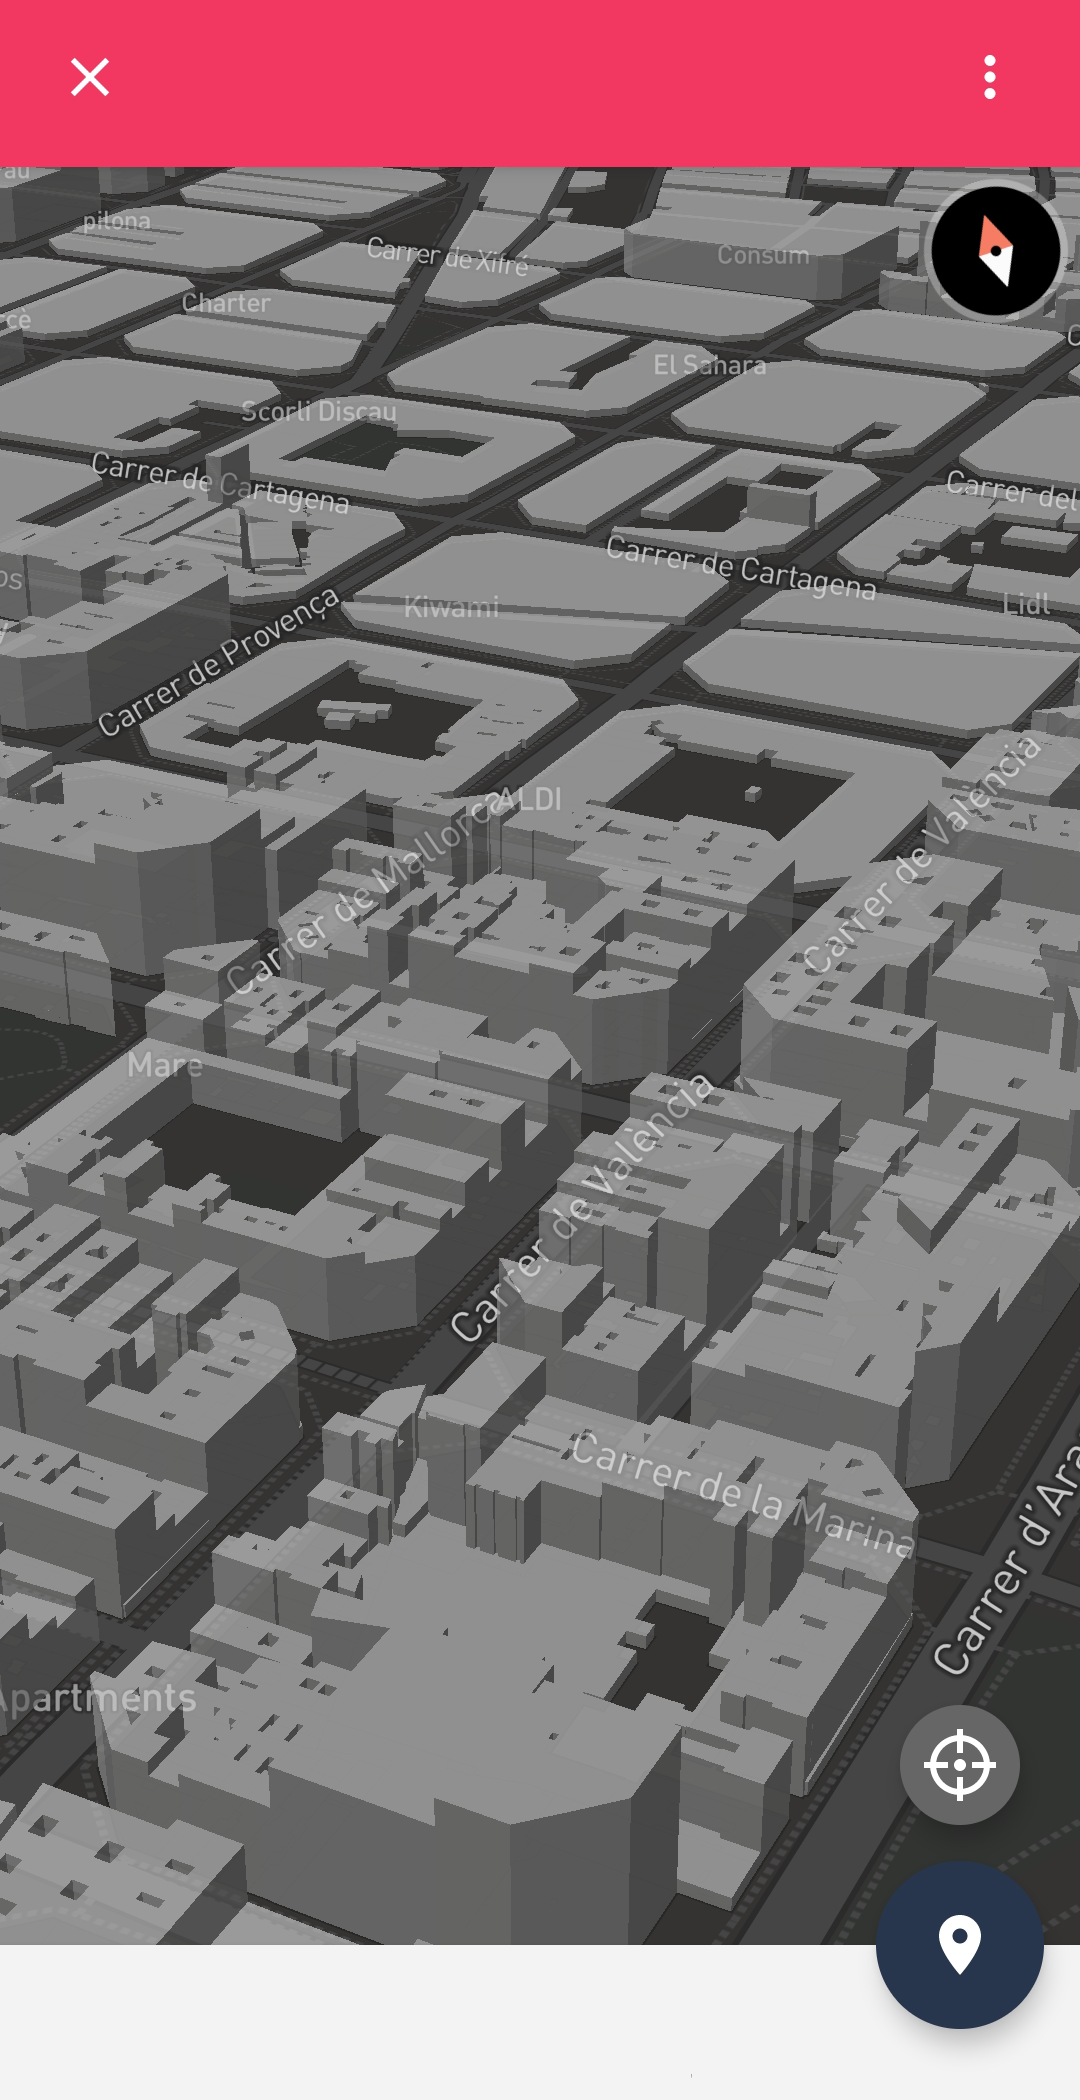
\includegraphics{figs/fundamentals/raster_gis.png}
	\caption{Vector data in a geographic information system within an Android application.}
	\label{fig:raster_gis}
\end{marginfigure}

\begin{figure}[!ht]
	\includegraphics{figs/fundamentals/raster_vectorial.png}
	\caption{Comparison of a) raster and b) vector representation of Vila Real District in Portugal.  }
    \label{fig:raster_vectorial}
\end{figure}

The spatial resolution of images refers to the number of pixels represented in $\mathcal{X}$ and $\mathcal{Y}$ axes. However, it can be further stressed to introduce the amount of space in \si{\meter^2} represented in a pixel. The latter is more frequent in \gls{Remote sensing}. It is typically derived from the image dimensions and the distance covered in $\mathcal{X}$ and $\mathcal{Y}$.

The most widespread impression of images is colour-space examples. However, there exists a considerable imagery taxonomy organized from the number of bands ($\mathcal{Z}$) and the information that is encoded in each of them. The literature's most revised kinds of imagery are visible (colour-space), thermographic, multispectral and hyperspectral. The sensors that capture this information are coined with the same name. In this regard, Figure \ref{fig:sensor_literature} shows the percentage of research devoted to each one of the mentioned tools in the last few years. Minority tools such as RGB-D, with D standing for depth, are omitted in this figure. The following sections delve into the results that are processed in this dissertation. 

\begin{figure}[!ht]
	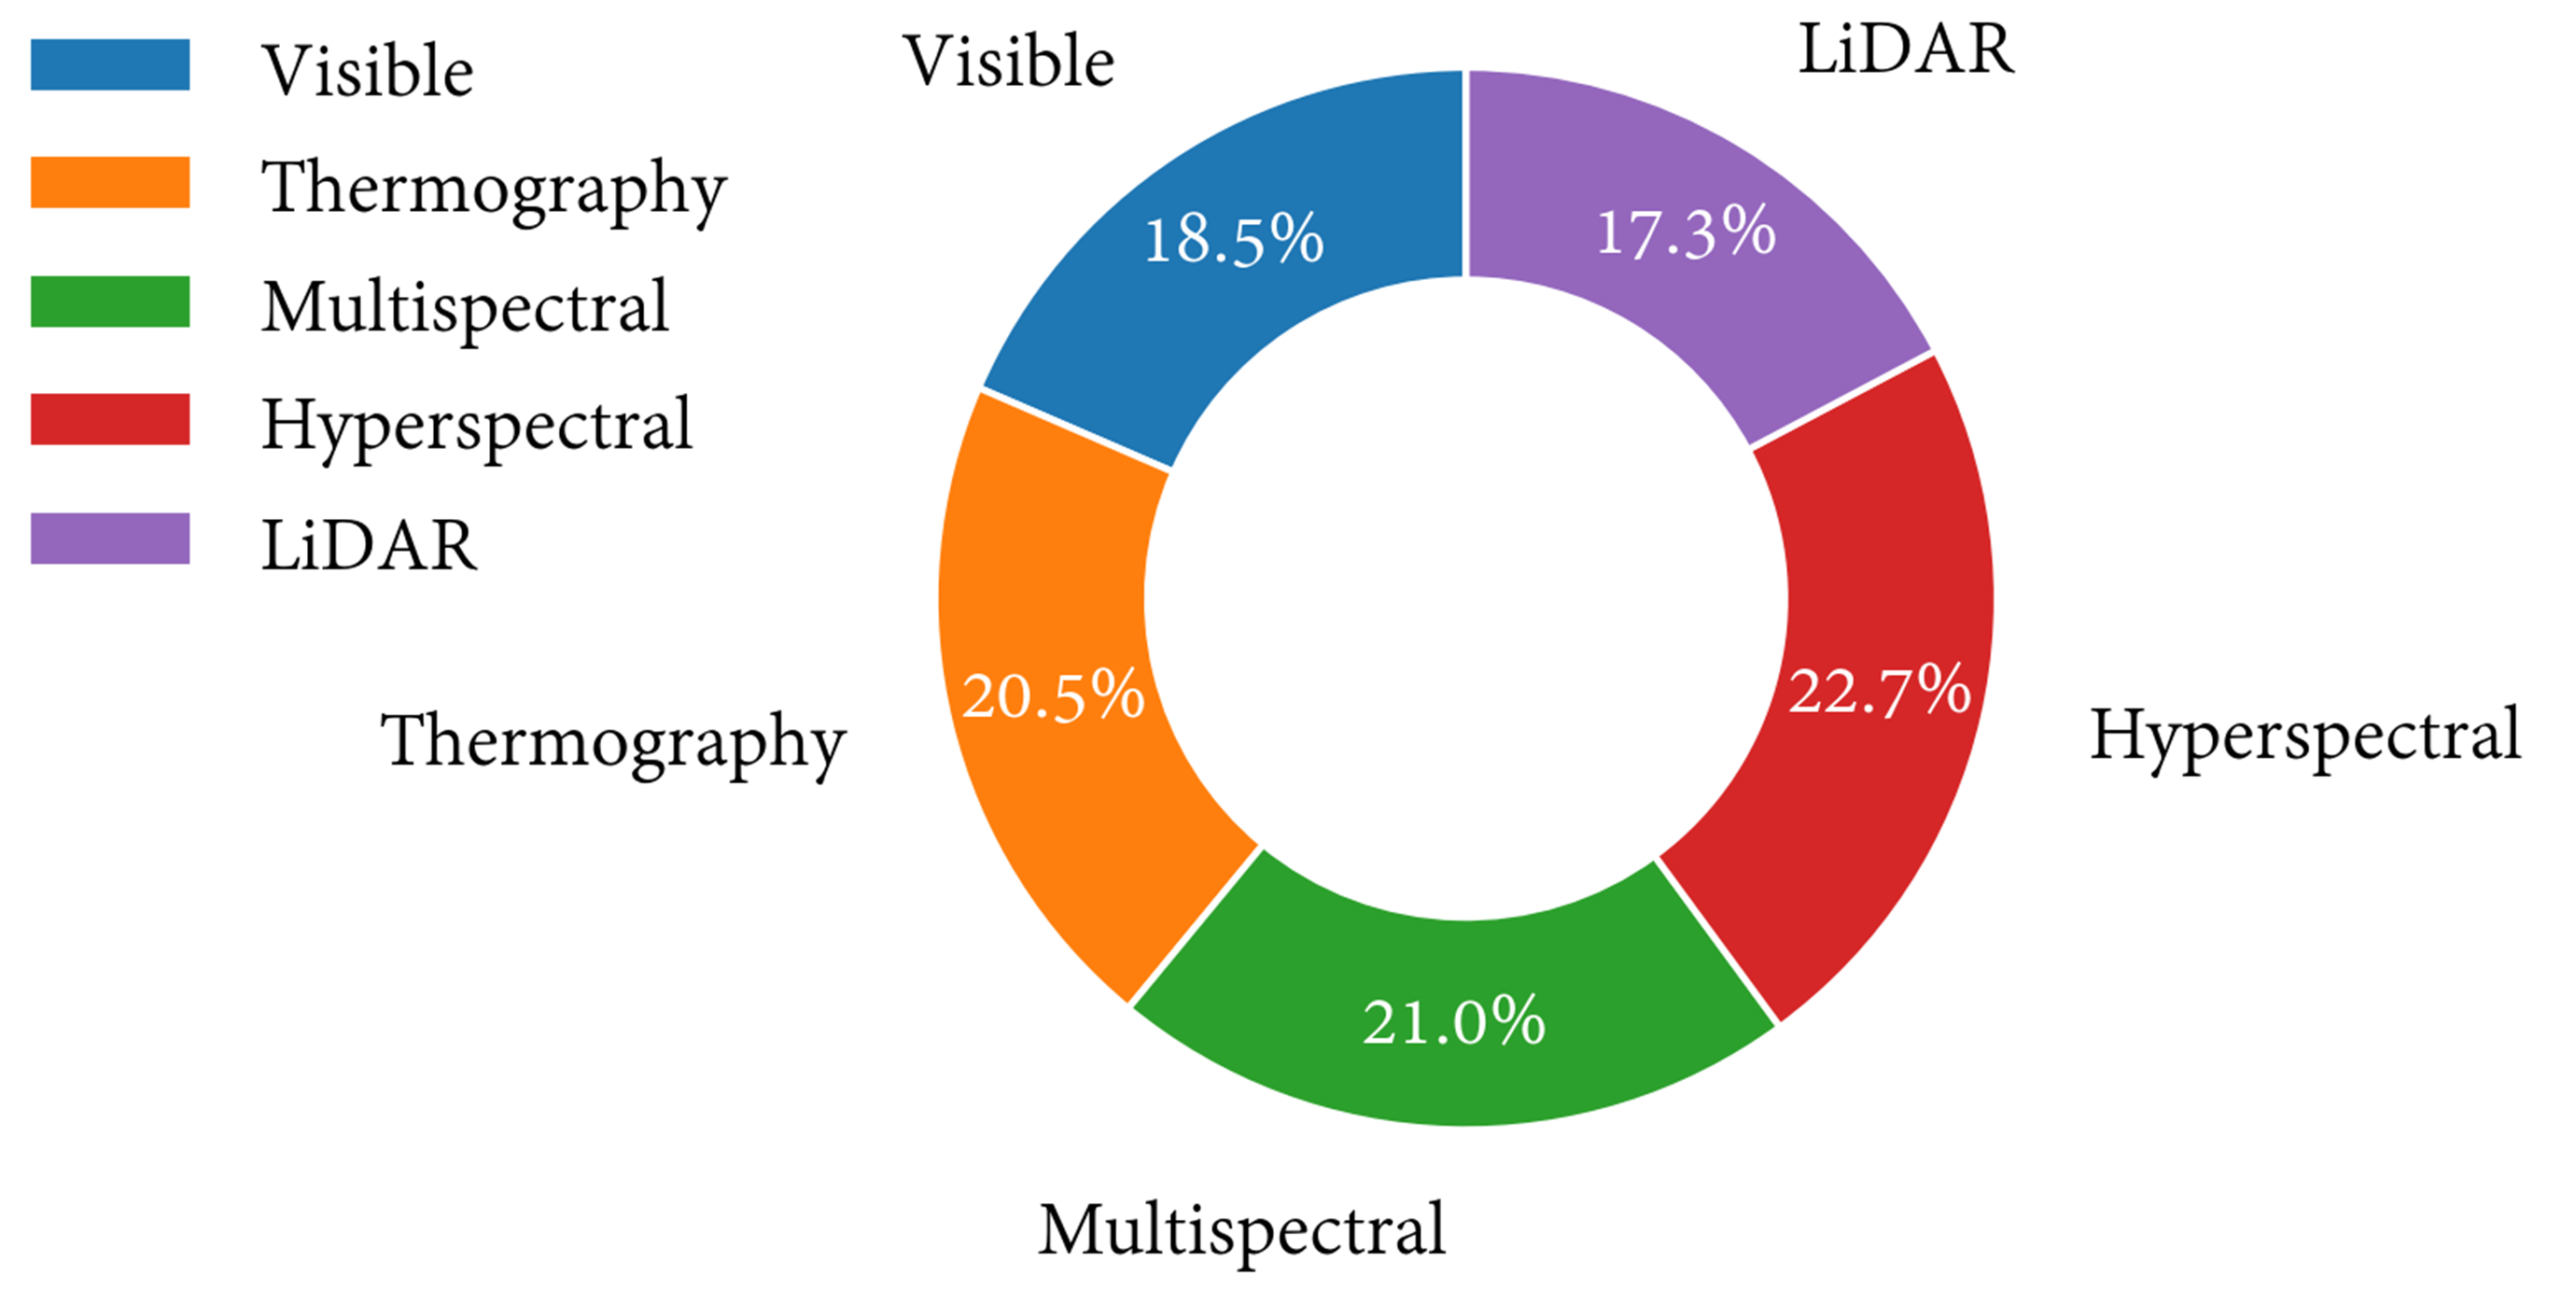
\includegraphics[width=.8\textwidth]{figs/fundamentals/literature_sensors.png}
	\caption{Comparison of a) raster and b) vectorial representation of the Vila Real District in Portugal.  }
    \label{fig:sensor_literature}
\end{figure}

\subsection{Point clouds}

Point clouds are collections of points with no connectivity, which are typically extracted from laser scanners and photogrammetry. There exists an enormous number of hardware and software solutions measuring real-world geometry at a constant pace, including the so-called digital twins. Although images carry relevant features and lead to meaningful conclusions, these are not linked to geometry. Three-dimensional representation of real-world scenarios has enjoyed a great interest to improve visualization and interpretation of the surveyed areas and phenomena. Therefore, 3D point clouds derived from imagery can be generated, if not directly acquired with passive sensing, to easier the view of target buildings, surfaces and any other area of interest. In contrast to 3D meshes, they enable a simpler, denser and more close-to-reality representation \cite{cao_3d_2019}. Besides the positioning, points can carry further information, including colour, reflectance, intensity, normal vector and classification label, among others. Additionally, all these values can be replicated at different timestamps throughout the time scale. Reviewing the scientific literature, it can be concluded that this problem is similar to that posed in the technique called projective texture mapping \cite{debevec_efficient_1998}–\cite{heckbert_survey_1986}. Initially, the aim was to have additional effects on the realistic image synthesis field of research, to cast shadows or render translucent objects \cite{dachsbacher_translucent_2003}.

The staggering pace of information acquisition and requirements concerning the level of detail of point clouds lead to massive 4D data, thus hardening the efficient storage, transmission and visualization. Yet, they are widely used in fields as disparate as autonomous driving systems, virtual and augmented reality, biomedical applications and precision agriculture. Geometric features provide further data that helps with the recognition and classification of objects, even for human operators. For instance, \cite{barros_multispectral_2022, kerkech_vine_2020, de_castro_3-d_2018} showed that elevation data significantly improved the classification accuracy on the segmentation of plots, with elevation being a derived product of photogrammetry and passive sensing. However, huge point clouds consisting of billions, even trillions of points, require up-to-date techniques that benefit from nowadays hardware, capable of massively working in parallel. The current state-of-the-art studies have extensively worked on the compression of point clouds, to save storage and reduce bit rate transmission, as well as on the efficient visualization of massive point clouds. 

Other operators such as the estimation of normal vectors will be following explored as it concerns a later chapter. However, this is simply a minimal part of research on point clouds, since the uncertainty from photogrammetry and laser point clouds must be individually addressed for each application. Part of this enormous amount of work comprises the classification, segmentation and identification of tree skeletons \cite{cardenas_reconstruction_2022} on point clouds. 

\subsubsection{Compression}

The huge amount of point cloud data represents a challenge both for storage and transmission. Furthermore, the following massively parallel operations are performed on GPU hardware with limited memory capacity. Although this drawback has been mitigated in the most recent GPUs (NVIDIA GeForce 40 series at the moment this dissertation is being written), these operations ought to work over commodity hardware. The most recent releases have a memory size ranging from 8 GB (GeForce RTX 3050) to 24 GB (GeForce RTX 3090, GeForce RTX 3090 Ti \cite{nvidia_nvidia_nodate-2} and GeForce RTX 4090 \cite{nvidia_nvidia_nodate-1}), whereas laptop models have typically their memory size reduced to half of these. Other high-performance GPUs focused on research, for example, NVIDIA A6000 \cite{nvidia_nvidia_nodate}, scale up to 48 GB and enable higher capacity using a bridge called NVIDIA NVLink. However, these high-performance products are not widespread, and most computers work using commodity hardware. Accordingly, GeForce Series 10 and 20 are less prohibitive, easier to acquire under stock shortage and more frequent to find in laptops not designed for high-performance tasks. The memory size of these devices is below 12 GB for Series 20 and 8 GB for Series 10. 

Furthermore, there exist frameworks for GPU visualization and computing that severely clamps the maximum buffer size. For instance, OpenGL has been the standard platform for visualization for decades. Version 4.3 introduced what is known as computer shaders, i.e., scripts solving small GPU tasks that can be massively parallelized. One would expect to be able to reserve buffers with a maximum size bounded by the GPU's memory capacity; however, this limit can be queried in OpenGL, showing the numbers in Table x.

Hence, massive point clouds require at some point to be compressed, mainly in transmission and visualization applications. This research field has been coined as PPC, Point Cloud Compression, distinguishing lossy and lossless methods. Similar to the computer science field, PPC has transitioned from traditional techniques \cite{bui_comparative_2021}, based on encoding using data structures (regular grids, octrees, kd-trees, etc. \cite{cao_3d_2019}) to Deep Learning, where the encoding is automatically learned by convolutional autoencoders (CNN-AE). The latter are more likely to lose data to some degree, unless the compressed data is discrete \cite{que_voxelcontext-net_2021}, such as octree nodes. 

Very few compression methods offer low-computational complexity for real-time transmission \cite{cao_3d_2019} and reconstruction (decoding), while others do not support the compression of colour information. However, \gls{Remote sensing} point clouds can carry large amounts of information for every point; from LiDAR points whose attributes follow the LAS file standard to hyperspectral points storing spectral signatures with hundreds of measurements. Rather than exploiting the point cloud's entropy in the spatial and temporal dimensions, \cite{graciano_quadstack_2021} proposed to compress layered datasets taking advantage of data redundancy. Although it was proposed to volumetric data from geology, biology or medicine fields, redundancy of sensor measurements can also be exploited for rendering. The algorithm is composed of three main steps: 1) stack redundant values on the $\textit{z}$ dimension to form the stack-based representation (SBR) from the initial heightfields, 2) group stacks with the same stack content (G-stacks) and 3) organize these into a quad-tree. Spatial redundancy is not as relevant for sensor data since it captures a wide variety of materials, whereas spectral compression is feasible at expense of downscaling the radiometric resolution. 

\subsubsection{Visualization}

Unlike triangle meshes intending to emulate continuous surfaces with underlying discrete polygons, point clouds are discrete representations. Therefore, visualizing the latter is tougher for scarce products with low point density. This hardens the detection of features and extraction of valuable information by human operators. Computationally, it implies increasing the neighbourhood distance from which features are extracted or simply leading to imprecise results due to the lack of data. The traditional rendering pipeline neither helps into accelerating the visualization of massive point clouds. It is designed for polygonal meshes that require 1) processing vertices, 2) including additional geometry, 3) discarding non-visible geometry, 4) rasterizing polygons, and 5) colouring polygon fragments \cite{akenine-moller_real-time_2018}.

The current state-of-the-art of massive point cloud rendering has evolved along with the impressive work of Schütz and Wimmer \cite{schutz_rendering_2019, schutz_rendering_2021}. The aim of their work was not only to speed up the visualization of billions of points but also to improve the rendered image. OpenGL's compute shaders were used to generate the images in the GPU and recently introduced NVIDIA extensions helped to further optimize it. An alternative rendering procedure is built over OpenGL to omit the stages 2), 3) and 4) of the traditional pipeline. In this work, vertices were massively projected into an image that is later rendered as a texture. However, the order in which points were projected into the planed showed to have a big impact on the performance. Points were transformed into Morton codes of 30 bits, 10 for every dimension, and sorted according to them. Then, globally sorted points were shuffled into small batch groups, whose size is determined by Graphic Processing Clusters (GPCs). Rather than distributing the work linearly, GPU organizes it into 2D patches assigned to GCPs. Thus, global sorting helps in grouping framebuffer updates, but it is suboptimal due to workload unbalancing. Spatially close GCPs in charge of visible points at a timestamp $t$ are assigned a heavy workload, while others remain idle. The random shuffling of globally sorted points using small batches was proved to slightly enhance the rendering performance.

\begin{figure}[!ht]
	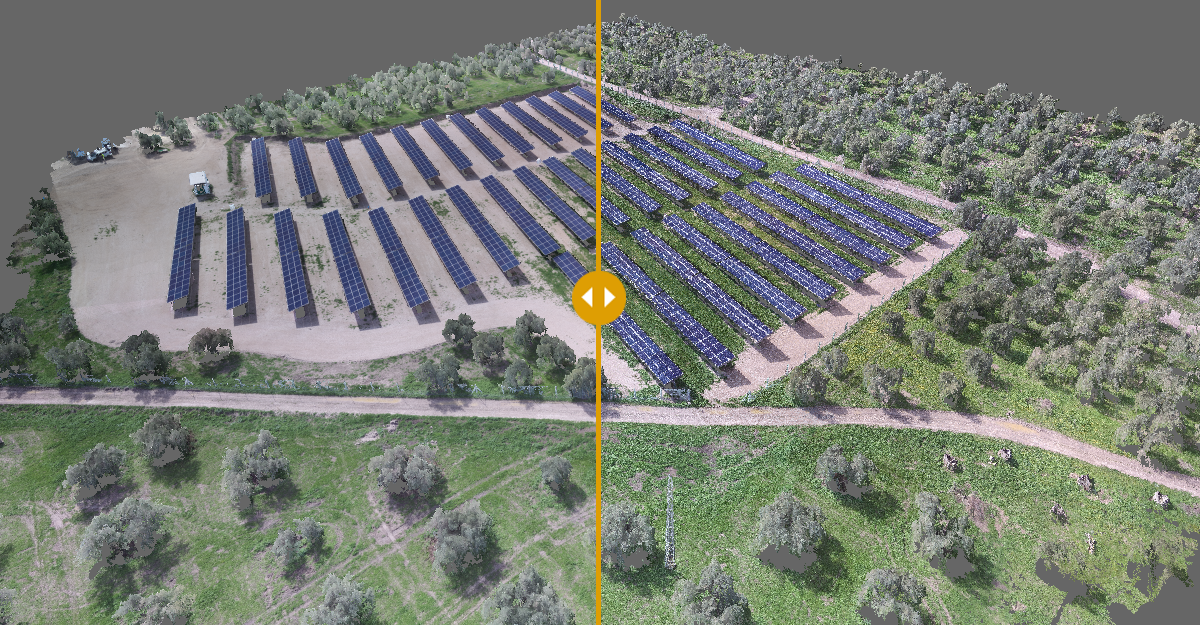
\includegraphics[width=\textwidth]{figs/fundamentals/hqs_comparison.png}
	\caption{On the left part, colouring using a mixed representation of surrounding points and on the right side, using a sole point colour for each pixel. This image was obtained using the procedure described by \cite{schutz_rendering_2021}. }
    \label{fig:hqs_pc_rendering}
\end{figure}

\begin{kaobox}[frametitle=Compute shader core proposed by Schütz and Wimmer]
The projection approach from Schütz and Wimmer \cite{schutz_rendering_2021} uses modern OpenGL extensions following this pipeline:
\begin{itemize}
    \item The depth buffer is firstly computed, with the depth being encoded along with the point index (64 bits). The atomic minimum operators help to select the point with the minimum depth. However, this approach leads to a noisy-like rendering for sparse point clouds. Instead, the depth of a pixel takes into account several points; data is exchanged within thread groups whose points fall in the same pixel using \verb|shuffleNV| and \verb|ballotThreadNV| operators. Then, \verb|shuffleXorNV| computes the minimum depth within a pixel neighbourhood.
    \item Colours are iteratively accumulated: the limited capacity of SSBOs may require that multiple point cloud subdivisions aggregate data. Accumulations can be implemented using atomic operators, whereas (red, green) and (blue, alpha ($\alpha$)) channels are encoded in two different buffers with values of 64 bits. Hence, the alpha channel is also used for accounting for the number of visible points at each pixel.
    \item Aggregated colours are finally transformed by averaging the mean value for each channel. Pixels with $\alpha \gets 0$ are coloured with the background tone. 
\end{itemize}
\end{kaobox}

Lately, optimizations of point cloud renderings have focused on the level of detail (LOD) and organization into Layered Point Clouds (LPC). A key in the construction of these data structures is that they ought to be view-dependent to enable adjusting the LOD based on the camera position and direction. \cite{schutz_gpu-accelerated_2023} proposed to index point clouds with octrees whose inner nodes are voxelized, whereas leaf nodes lead to the point primitives. \cite{ogayar-anguita_nested_2023} managed to create an adaptive hierarchical structure that coupled different data structures at different levels. It was shown to retrieve larger amounts of points with higher average and peak throughput. Previously, \cite{schutz_software_2022} sorted points with their Morton codes, split them into batches and built a hierarchical data structure using these batches as leaf nodes. Visualization of LODs varies according to the camera, and therefore, patches of different point densities could be rendered for distant objects. If the underlying discrete levels of a LOD-based data structure are visible, they are referred to as rendering artefacts. \cite{van_oosterom_organizing_2022} proposed to organize point clouds into a Space Filling Curve (SFC) and compute the continuous LOD of every point, thus enabling gradual changes in the point density. 

Noise in point cloud visualization was mitigated by \cite{schutz_rendering_2019, schutz_rendering_2021} using modern OpenGL extensions. Individual GPU threads are grouped in subgroups, also known as warps, of size 32 in NVIDIA microarchitectures, that can communicate efficiently and exchange results. For a globally sorted point cloud, warps work over spatially close points that can aggregate colour data. Hence, this approach leads to the High-Quality Shading (HQS) variant proposed in \cite{schutz_rendering_2021}, thus providing a more continuous shading (see Figure \ref{fig:hqs_pc_rendering}). This also opens the possibility of filling holes derived from lower point density rather than reconstruction failures. 

\subsubsection{Occlusion detection}

The projection of additional sources of information over point clouds is trivial once camera poses are estimated. For each viewpoint, the camera matrix enables the projection of 3D points into the image plane. However, projections do not separate background and foreground surfaces; although a point may be theoretically visible from a camera, it could be covered by another surface in the real scenario. The chances are that points are visible in more than a single viewpoint, and therefore, erroneous assignments of information may be partially masked by other correct measurements. However, this approach is not precise for colouring point clouds and occlusion must be detected to tackle this.    

\begin{marginfigure}[3cm]
	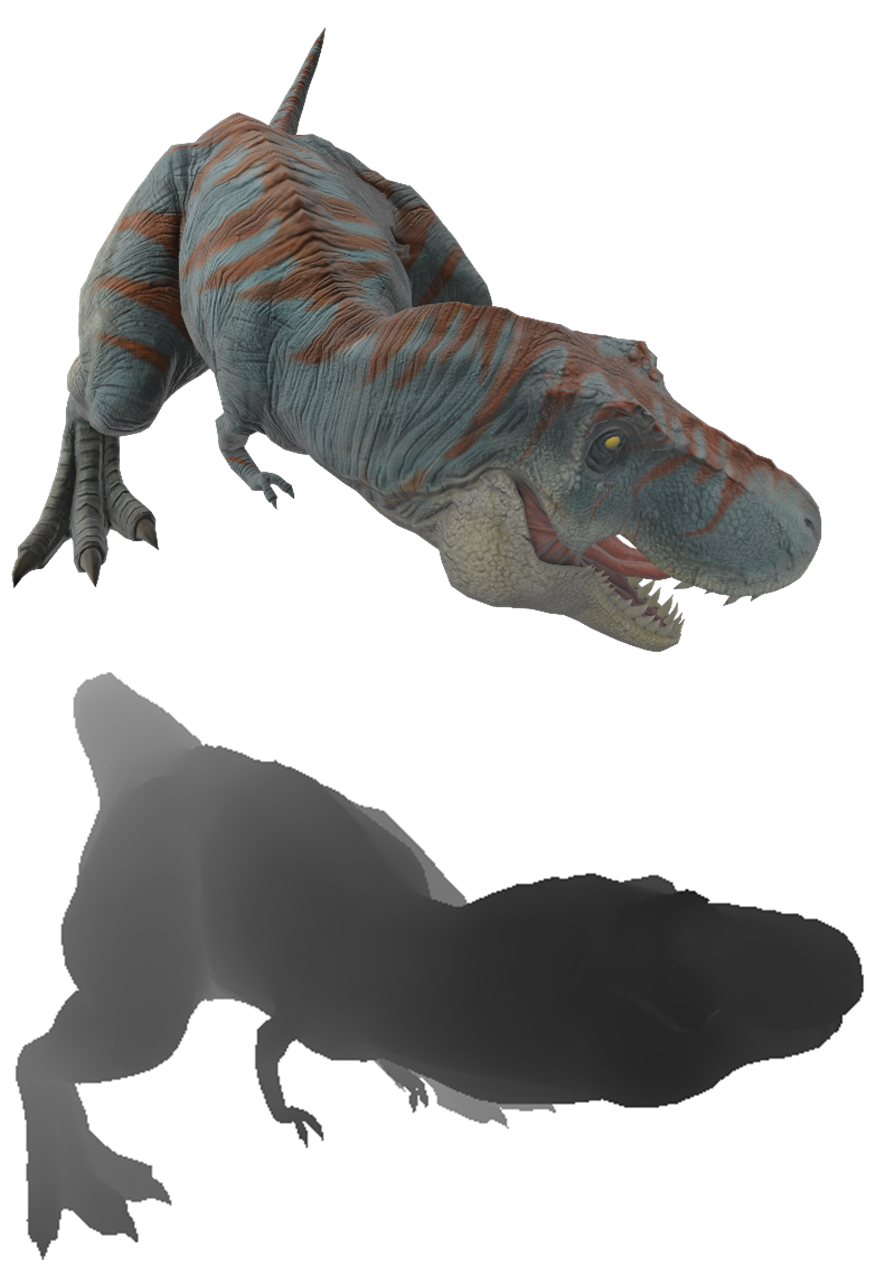
\includegraphics{figs/fundamentals/z-buffer.png}
	\caption{Vector data in a geographic information system within an Android application.}
	\label{fig:z-buffer_opengl}
\end{marginfigure}
The most straightforward way to detect occlusion is to use what is called $z$-buffers in rendering: images that store for each pixel the minimum depth at which geometry was projected. It has been traditionally used for shadowing and discarding non-visible geometry for optimizing the rendering \cite{akenine-moller_real-time_2018, white_cascaded_2021}. Similarly, it enables recording the nearest visible point at every image's pixel. It does not require indexing points into a data structure, though they are of great help to narrow the subset of points to be projected into a single viewpoint. Determining the nearest depth is trivial in the GPU, as most GPGPU frameworks provide atomic operations. Despite these being supposedly slower operations, they compete well against other approaches in terms of memory consumption and efficiency. \cite{jurado_out--core_2022} proposed to build out-of-core occlusion-aware multispectral point clouds in CUDA. Asynchronous data loading and computation were applied to complete $z$-buffers for hundreds of images and point clouds of up to 1,084M points. Instead of using $z$-buffers, \cite{jo_dense_2021} computed the point and camera distance to solely project information from the closest viewpoint. This approach leads to errors if the point remains occluded from the closest one, though it can work over very dense and uniform image datasets. Not to mention this colour assignment is more prone to noise, while aggregations mitigate it. 

\begin{figure}[!ht]
	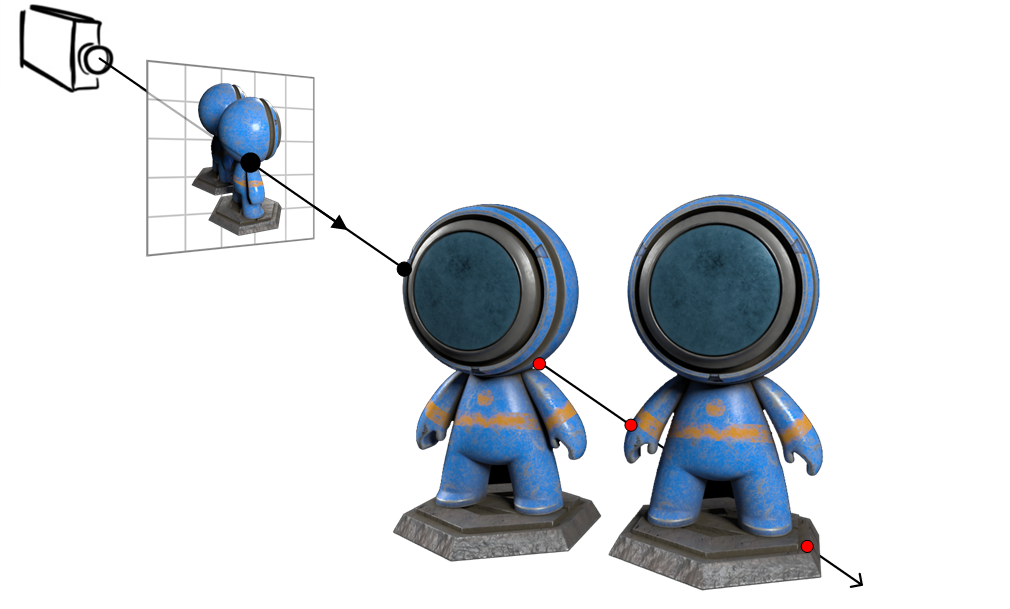
\includegraphics[width=\textwidth]{figs/fundamentals/occlusion.png}
	\caption{Occlusion of left figure over the right one on a projection made from the left part of the scene. }
    \label{fig:occlusion_concept}
\end{figure}

An alternative to $z$-buffers is to estimate the underlying polygon mesh of point clouds. In this regard, occlusion can be detected by constructing a small triangle mesh from points surrounding the main one \cite{jurado_multispectral_2020}. The point neighbourhood was sought using k-nearest neighbours (KNN). Although this method may achieve good results over planar surfaces, polygonal meshes are harder to reconstruct in other scenarios, for example, forestry with dense, and incomplete, vegetation. Other studies benefit from additional sources of information to detect occlusion, such as the semantic segmentation of point clouds \cite{schneider_fusing_2010}. 

\subsubsection{Photogrammetry}

Photogrammetry refers to the science and technology of generating geometrically correct products derived from photographs. 3D reconstructions are fundamental in this dissertation, as they provide an automatic procedure for modelling scenes, in contrast to Computer-Aided Design (CAD) tools, arm-mounted probes and active methods. However, mapping is also derived from what was coined as photogrammetry: the fusion of image datasets to compound results that helps in the understanding and visualization of target areas. Some of the most common maps are Digital Surface Models (DSM), Digital Terrain Models (DTM) and orthophotos. These products are estimated from datasets ranging from UAV-based imagery, which is known to be acquired sequentially in most cases, and large datasets from publicly available data. The latter images are harder to manipulate since one of their major stems is crowd-sourcing from the Internet: data published by users with very different devices, lighting conditions, objects present in the scene, etc.

The transition from laboratory to outdoor was possible due to the advent of digital images with higher resolution, better computational capabilities and mature techniques. The overall procedure in photogrammetry is 1) to estimate parameters from cameras, 2) to reconstruct 3D points and 3) to reconstruct materials if necessary. Two slightly different techniques have had great success in recent years: Structure from Motion (SfM) and Visual Simultaneous Localization and Mapping (VSLAM), though this section is focused on the first. 

The SfM method comprises a vast literature, but it has been robustly applied for over 20 years. The basis consists of 1) detecting key points in images, 2) matching these key points among multiple images, 3) estimating camera parameters from previous links and 4) building SfM models. The final step, despite not being part of SfM, is to reduce errors from estimations, also known as bundle adjustment (BA). The error to be minimized is formally defined as follows (Equation ):
\begin{gather}
    \label{eq:error_bundle_adjustment}
    \begin{aligned}
        E(P, M) = \sum_{j} \sum_{i \in V(j)} \mid P_i(M^j) - m_{i}^{j} \mid^2
    \end{aligned}
\end{gather}
where P is a set of camera parameters, ${P_i}$, $M^j$ represents a set of 3D coordinates of a track, $m_{i}^{j}$ are the projections of $M^j$ in the i-th camera, $V(j)$ are the list of caneras where point $M^j$ is visible and $P_i(M^j)$ is the projection obtained by using the camera parameters $P_i$.

SfM is also found in the literature as SfM-MVS, with MVS referring to Multi-View Stereo. MVS originated as an improvement to two-view stereo algorithms. Instead, thousands of images are applied to the reconstruction of large metropolitan and natural scenes. However, the main concerns in this regard are the photo-consistency of features that are identified in several images. As we previously stated, conditions may vary from one viewpoint to another; hence, it is required to calculate how likely a candidate in $V_i$ is the correct match of a pixel in $V_j$, with $i \neq j$. Finding candidates for every feature over huge datasets is neither trivial nor efficient. Therefore, most of nowadays photogrammetric software is programmed in the GPU to accelerate the pipeline.

Applying photogrammetry is not prohibitive, and it is even possible to find mobile-based applications that can work over cost- and time-efficient imagery recorded on mobile phones. Computer-based solutions, aimed at large datasets, include open-source and commercial software. The first group includes ColMap, AliceVision, Zephyr and VisualSfM, whereas notable commercial software includes Pix4DMapper \cite{zheng_thermal_2020}, Agisoft Metashape \cite{grechi_3d_2021}, RealityCapture and Autodesk Recap 360 \cite{lafi_3d_2017}. The first two commercial solutions are sped-up using multi-core CPU and GPU acceleration for image matching, whereas BA is performed in the CPU. \cite{jiang_efficient_2020} revised the efficiency of SfM implementations by applying it over four datasets. According to their evaluation, performed using commodity hardware, Metashape showed the worst performance both for BA and feature matching, whereas RealityCapture showed similar performance during feature matching and significantly better during BA. However, Agisoft Metashape generated the densest point clouds for every dataset. Also, reported results on the literature depends on the computer used during the experiments and yet, they may vary over a short period of time. For example, Agisoft Metashape is currently known to support accelerated processing in the GPU for image-matching, depth-map reconstruction and other mesh-related operations. It works over CUDA-enables GPUs, and hence, it was not expected to provide results as discouraging as reported by \cite{jiang_efficient_2020}.

\subsubsection{Colour aggregation}

A final remark must be done on colour aggregations. Points receive multiple values that may vary one from another since these are captured under different lighting and viewing conditions. The observed radiance varies according to the viewing angle, expressed through azimuth, $\phi \in [0, 360]$, and zenith, $\delta \in [0, 180]$, angles. Also, surfaces behave so that the emitted radiation is not spread uniformly unless it is a perfect Lambertian generator \cite{vollmer_infrared_2017}. Hence, surfaces emit more radiation if $\delta = 0$, i.e., the camera's view vector is $-\hat{n}$, the normal vector of the surface. The naïve and widespread way to solve aggregations is to average them \cite{javadnejad_photogrammetric_2020, hoegner_3d_2016}, while consensual approaches minimize the distance from the aggregated value to the originals. The latter method has been mainly applied to expert-guided decision-making to aggregate opinions following those operators that minimize the conflict among the experts' views.

Instead of averaging samples, multiple aggregation functions can be used together with penalty functions to select that provides the result which differs less from the experts' opinions. In this context, experts are different camera viewing angles obtaining distinct results. The use of penalty functions is on computing the similarity of each aggregation and the starting samples \cite{bustince_definition_2017, bustince_penalty_2017}, which must be maximized. Although penalty functions have been gaining interest in scientific research, they have barely been explored in some contexts such as image processing \cite{paternain_color_2012}. 

\begin{figure}[!ht]
	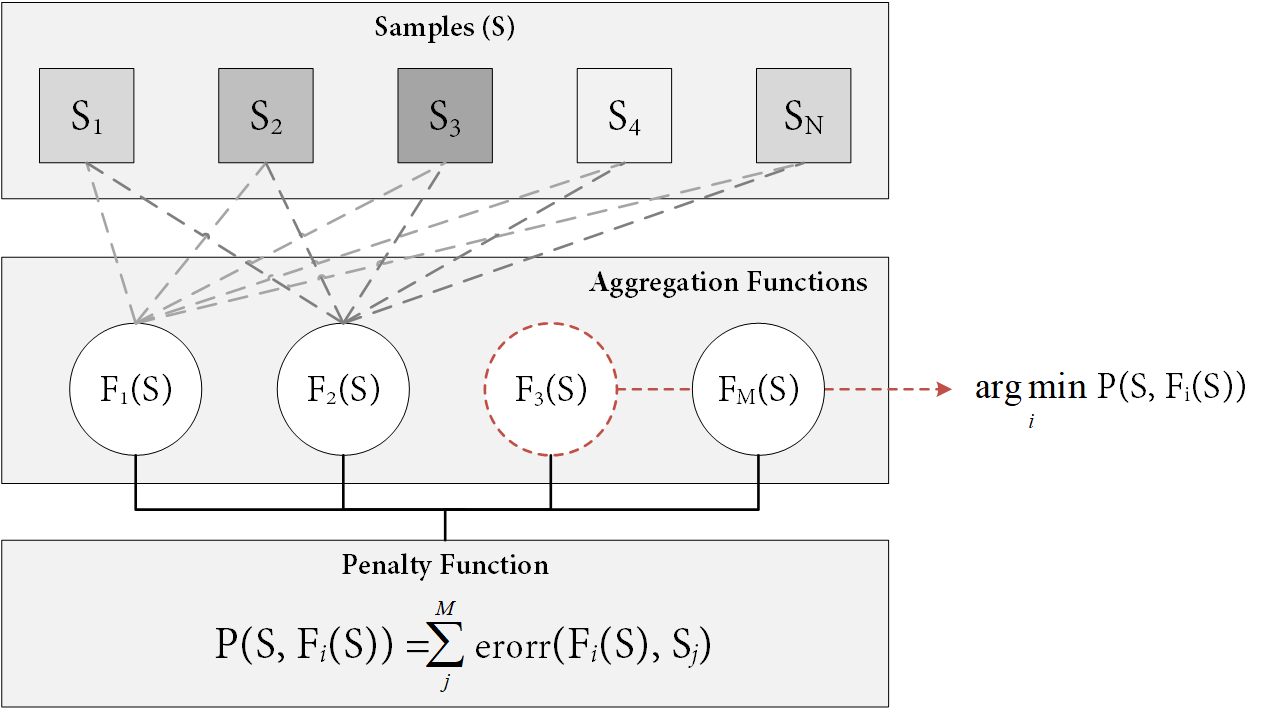
\includegraphics[width=\linewidth]{figs/fundamentals/penalty_functions.png}
	\caption{Overall procedure to compute the penalty value of every available aggregation.}
	\label{fig:penalty_funtions}
\end{figure}
Briefly, n-ary aggregation functions, $f: [0, 1]^n \rightarrow [0, 1]$ are monotone increasing and satisfy the boundary conditions (Equation \ref{eq:aggregation_boundary1}).  
\begin{gather}
    \begin{aligned}
        &\forall i \in \{1,...,n\}, \hspace{1mm} x_i \leq y\\
        &\Rightarrow f(x_1,...,x_n) \leq f(x_1,..., x_{i-1}, y, x_{i+1},...,x_n)\\
        &f(x_{\textit{min}},...,x_{\textit{min}}) = x_{\textit{min}}\\
        &f(x_{\textit{max}},...,x_{\textit{max}}) = x_{\textit{max}}
    \end{aligned}
    \label{eq:aggregation_boundary1}
\end{gather}

On the other hand, averaging aggregation functions are bounded by the minimum and maximum input (Equation \ref{eq:aggregation_boundary2}).
\begin{gather}
    \label{eq:aggregation_boundary2}
    \begin{aligned}
        \textit{min}\{x_1,...,x_n\} \leq f(x_1,...,x_n) \leq \textit{max}\{x_1,...,x_n\}
    \end{aligned}
\end{gather}

Finally, penalty functions, $P: \R^{2} \rightarrow \R$, satisfy the conditions in Equation \ref{eq:penalty_conditions}, where \textit{y} is the aggregated value. Consequently, penalty functions can be expressed as $\sum_{i=1}^{n} P(x_i, y)$ with the goal of retrieving the aggregation that minimizes the value of $P$, $g(x) \gets \operatorname*{argmin}_y P(x, y)$.
\begin{gather}
    \label{eq:penalty_conditions}
    \begin{aligned}
        &P(x_i,y) = 0 \hspace{2mm} \forall x_i = y\\
        &P(x_i,y) > 0 \hspace{2mm} \forall x_i \neq y\\
        &P(x_i,y) \ge P(x_j,y), \hspace{1mm}\mid x_i - y \mid > \mid x_j - y \mid\\
    \end{aligned}
\end{gather}

\subsubsection{Normal estimation}

Point clouds, either derived from photogrammetry or passive sensing, lack certainty in most of the attributes that provide further value to this product, ranging from normal vectors to semantic labels of different levels of detail. Many studies work on solving the uncertainty of these attributes, where normal estimation is a recurrent topic. This operation is provided as a ready-to-use tool in some widespread libraries for point cloud processing, for example, PCL (Point Cloud Library) and CGAL (Computational Geometry Algorithms Library). Since these are very time-consuming tasks, implementations are even facilitated as multi-core solutions that significantly reduce the latency. 

Most methods addressing normal estimation operate over neighbourhoods of varying dimensionality that correlate points to form minimal triangle meshes, from which normal vectors are estimated. Thus, the main challenges in this procedure are selecting an appropriate neighbourhood size and noise resilience, as these factors greatly contribute to wrong estimations. From the neighbourhood, plane fitting is approached using unweighted Principal Component Analysis (PCA) and Singular Value Decomposition (SVD). Another challenge is the efficiency of the method: seeking the nearest $n$ points is not trivial nor efficient unless memory-consumpting data structures are built into point clouds. Hence, some works have proposed to perform a global sort on the basis of Morton codes calculated from $\textit{xyz}$ coordinates \cite{jakob_optimizing_2021}. This way, the neighbourhood is narrowed to spatially close indices on a linear buffer.

With current trends in AI, normal estimation has also been achieved with Deep Learning techniques. It can be achieved by representing point clouds as graphs \cite{lenssen_deep_2020} and images \cite{zeng_deep_2019, boulch_deep_2016} since it must be performed per point rather than per voxel. To this end, additional sources of information such as depth and Hough transform \cite{boulch_deep_2016} help with the normal estimation along with $\textit{xyz}$ coordinates. 

\subsubsection{Parallel processing}

This section is focused on the revision of approaches for parallelizing processes concerning \gls{Remote sensing}, rather than on specific applications. The key term in this brief section is GPGPU, General-Purpose computing on Graphics Processing Units, which is a programming field that takes advantage of GPUs to rapidly solve parallelizable tasks. This is possible due to the large number of cores this hardware comprises. 

In this regard, OpenGL (OpenGL Graphics Library) is the most widespread solution since it allows both rendering and solving computing tasks using massive geometry. From a rendering approach, point clouds have their own primitive in the draw calls, \verb|GL_POINTS|. It follows the standard rasterization pipeline while processing point clouds for rendering, despite some of these are not required for such a primitive. This drawback can be sorted out with other already explained approaches implementing a custom pipeline \cite{schutz_rendering_2021, schutz_software_2022}. For problems involving parallel computing and rendering, OpenGL is an easy-to-use platform as it allows developers to resolve both tasks at once. However, one of the main shortcomings of GPGPU OpenGL is the handling of asynchronous tasks that could overlap to get the most out of the GPU's capabilities, which is very limited in OpenGL and constrained to the use of barriers. More recently, OpenGL has been discontinued at expense of more efficient and adaptive graphics frameworks such as Vulkan, which are expected to turn into the standard frameworks in this field. Since these are still ongoing and remain niche, very few works use these platforms \cite{stumpfegger_gpu_2022}.  

Another standard framework for GPGPU is CUDA. As opposed to OpenGL, it is not a cross-platform tool; instead, it is only able to operate over NVIDIA GPUs, but it also provides a more flexible GPGPU framework. With OpenGL being discontinued, most GPGPU studies that used OpenGL has transitioned to CUDA over time \cite{schutz_gpu-accelerated_2023}. Nevertheless, recent NVIDIA extensions have been introduced on both platforms. Other GPU-based rendering and computing platforms are DirectX \cite{baek_accelerated_2020} (Windows OS), OpenCL (cross-platform) and Metal for Apple platforms. 

\subsubsection{Fundamentals of optical imaging}

The underlying concept in \gls{Remote sensing} is to measure the emitted energy from the Earth's surfaces either from excitation of internal processes or interaction with incoming energy. We refer to energy as electromagnetic (EM) radiation that travels through time and space with a wave-like shape. If these are unpolarized, they oscillate in all the directions that are perpendicular to the travelling vector. The number of oscillations is known as frequency ($\nu$), whereas the spacing between two successive crests is the wavelength, $\lambda$. In a vacuum, EM radiation travels at the speed of light, $c = \lambda * \nu$; in nature, it depends on the traversed medium. The fundamental unit in EM radiation is the photon, the physical form of a quantum, and these units are the target of the following described optical imaging tools \cite{emery_introduction_2017}. These are designed to capture EM radiation passing through a polarized filter, thus focusing on a specific spectral interval.

The early cameras were simply light-tight boxes with a pinhole from where the light was allowed to pass through. The exposure of the film was controlled by letting light pass or not through it. Then, they were replaced by lens cameras aimed at enlarging the hole, thus capturing more light in less time. Besides lenses, these systems were also composed of a diaphragm adjusting the diameter of the lens opening, $d$, and a shutter that controlled the exposure time. Nowadays cameras are not different from early simple lens cameras, though focus and exposure must be properly controlled. In this dissertation, the focus is on sensors measuring EM radiation as functions of location ($x, y$), time ($t$) and wavelength ($\lambda$). These sensors are classified into imagers, which produce two and three-dimensional images, and nonimagers, such as hand-held devices that output single response values. 

Imagers are also known as radiometers, and these instruments require decomposing the radiation contributions and quantifying them with matched detectors. The first dispersion method is a prism, which was first utilized to separate out wavelengths by Isaac Newton. This dispersion results from refractivity being dependent on wavelength, causing entering light rays to exit at different angles. Other dispersion mechanisms are filter-wheel radiometers, grating spectrometers and interferometers, where the former is the most widespread. Filter-wheel radiometers separate wavelengths using a wheel, composed of radiative filters, that cycles through the radiation path. Filters can be classified as absorption- or interference-based, though only the first is integrated into a filter-wheel. They can be designed to pass long, short or very narrow wavelength bands, defined by a central wavelength and  cutoff limits. Coloured absorption filters are made of coloured glass or dyed gelatin that absorbs energy from a wavelength interval and let others pass. Furthermore, filters also attenuate the passing radiation, and their radiative efficiency is given by the signal-to-noise ratio (SNR).

On the other hand, the transmitted energy must be captured into images. The transition from analogical to digital photography was led by utilizing solid-state sensors instead of silver halide crystals, with the first being more sensitive to brightness changes. Digital cameras incorporate two-dimensional arrays of semiconductors, either charge-coupled devices (CCD) or complementary metal-oxide (CMOS). Each one of these detectors is dedicated to sensing the energy for an image's pixel. The scene brightness captured in that pixel is proportional to the small electrical charge triggered by the striking energy. Charges are transformed voltages values using the photodetector's area and responsivity, the incoming radiance and the spectral width, followed by A-to-D conversion. Although semiconductors are monochromatic, RGB-colour data can be obtained by placing filters over these photosites in the sensor array with a Bayer pattern. Red, green and blue photosites are arranged so that missing colour data can be interpolated from surrounding photosites with the same colour. With this pattern, half the filters are green, while the remainder is equally split into blue and red. Other detectors are able to record red, green and blue radiance at every pixel, such as Foveon CMOS \cite{lillesand_remote_2015}. Besides RGB, hyperspectral imaging constitutes a challenge as it does not require capturing three simultaneous wavelengths, but hundreds of narrow bands. Hence, photo-detectors are arranged as arrays along the spatial and spectral dimensions. Depending on the wavelength range, the material in which semiconductors are made varies; from silicon (visible) to PbS (lead sulfide, near-IR) or InSb (indium-antimony, mid-IR). 

The overall objective of imaging spectrometers is to observe large portions of the Earth and therefore, to progressively build data cubes recording spectral and spatial information. However, it is possible to scan the area of interest with hundreds and thousands of images or simply with a few of them that are built as the scanning platform translates, thus yielding larger images than usual. 

\subsubsection{Scan geometry}

At least three scanning geometries are distinguished, involving different mechanical and optical principles: single-snapshot, whiskbroom and pushbroom.

Single-snapshot is the most widespread scanning geometry. Matrices of semiconductors simultaneously acquire spatial and spectral information of the area of interest. Therefore, there is no scanning involved; it captures a single snapshot with limited spatial resolution. The main drawbacks are given by the dimensionality of CCD arrays, as it bounds the number of pixels. Although it is possible to increase spatial or spectral resolution by enlarging CCD arrays, it may come at the expense of reducing the dimensionality of one axis. This is especially relevant for imaging devices producing large data cubes, e.g., hyperspectral. Despite the advent of large detectors measuring millions of voxels at the same time, the already huge size of hyperspectral CCDs forbids enlarging axes without penalizing others \cite{sousa_uav-based_2022, pu_hyperspectral_2017}. 

On the other hand, push-broom or line-scanning is possible with a 2D matrix of semiconductors ($\lambda \times x$) recording data in the spectral, $\lambda$, and spatial, $x$, dimensions. Due to the CCD array being 2D, horizontal sweeps are acquired simultaneously (lines), and these are accumulated into images known as swaths. Thus, this approach requires a mobile platform or imaging device that moves forward and helps to enlarge the observed area in $y$. Rather than a complex mechanical system, this scanning requires an optical design that collects radiation with pointing mirrors and collimates it into dispersing elements \cite{sousa_uav-based_2022, pu_hyperspectral_2017}. 

Whiskbroom geometry is halfway into single-snapshot and push-broom. The core of this approach is a rotating mirror that dispersers radiation through a grating plane or prism into a linear CCD array with dimensionality $\lambda$. Hence, it requires a lesser number of photo-detectors than previous geometries and consequently, these devices are easier to calibrate while providing a high spectral resolution and radiative sensitivity. Due to the acquisition mechanism, the dwell time on every pixel is also smaller, which leads to a lower Signal-to-Noise Ratio (SNR). However, the misalignment of bands in single-snapshot and lines in push-broom is here found at the pixel level, thus hardening the generation of orthorectified products \cite{pu_hyperspectral_2017}.

Besides the scanning geometry, aerial photographs are taken along flight lines and thus their acquisition setup also matters for final results. First, these are recorded along a viewing direction, with $\textit{nadir}$ being the most trivial, i.e., perpendicular to the soil represented as a horizontal plane. Furthermore, successive images are taken with a degree of overlapping, either end lap or side overlap. It guarantees that features are visible in more than one image, thus leading to stereoscopic pairs and stereoscopic coverage. End lap revers to overlapping between successive images in the same flight strip, whereas side overlaps count for the overlapped in consecutive strips. The geometric elements of a vertical photograph are straightforward, considering that $o$ is the principal point, the interception of the optical axis with the film plane, and that the optical axis governs the view direction. In Figure \ref{}, the photograph is taken in nadir.

\subsubsection{Multispectral imaging}
\label{sec:multispectral_imaging}

Multispectral images consist of multiple bands corresponding to different wavelengths. However, these are typically discrete readings of spectral intervals with varying bandwidths. Most of the research and academic work describe multispectral as a special case of super spectral and hyperspectral imagery, and so we will, though some remarks are mentioned in this section for our later work. First, Table \ref{table:multispectral_devices} presents some of the multispectral sensors that are frequent in the literature, along with the works where they were mentioned. The discrete wavelengths and the resolution of every reading are shown in the fifth column, Spectral bands. It can be observed that only a few bands are recorded with coarse resolution, ranging from 14 \si{\micro\meter} to 57 \si{\micro\meter}.

\marginnote[3cm]{For tasks such as vegetation classification, visible and near-infrared bands from multispectral imagery are sufficient in most cases. Bare soils tend to show a more constant spectral signature, whereas vegetation presents a steeper slope and thus higher values for near-infrared wavelengths \cite{navulur_multispectral_2006}.}
The most frequently recorded bands are Red, Green, Blue, Red-edge (REG) and Near-Infrared (NIR), thus overlapping with previous and later imaging tools (visible and thermographic cameras). REG bands are halfway between Red and NIR, while NIR overlaps with Longwave Infrared (LWIR) wavelengths. Despite other sensors being able to capture most of these individual bands, multispectral imaging opens a wide number of opportunities by simultaneously recording bands sparsed throughout the visible and infrared spectrum. Most of the multispectral applications benefit from multiple bands through the so-called indices, i.e, linear combinations of them aimed at highlighting relevant features in a group of target objects. In this regard, a total of 82 spectral vegetation indices were collected from the literature by Pu, Ruiliang \cite{pu_hyperspectral_2017}. A recurrent vegetation index in Precision agriculture work is NDVI (Normalized difference vegetation index), calculated as a combination of Red and NIR bands. Besides identifying vegetation, other indices are focused on estimating pigments and chlorophyll content in plants \cite{pu_hyperspectral_2017}. Most of them work by aggregating bands where the target compound has the most and less significant presence, while others are rather aimed at simply detecting its presence despite obtaining a real value.

However, the revision of vegetation indices converges into the previously mentioned shortcomings of multispectral imagery. Most of these indices operate very specific wavelengths, e.g., $670, 800, 1050$, etc., while only a few bands are captured in multispectral imaging. Although it is possible to approximate missing wavelengths with the most similar bands, the results are far from optimal. Therefore, multispectral imaging is better suited for trivial applications such as vegetation classification, while it is not sufficient for other applications that require lower spectral resolution, such as mineral mapping or classifying vegetation species \cite{navulur_multispectral_2006, pu_hyperspectral_2017}. Indeed, most of the metrics proposed in the literature for discerning spectral signatures are based on its derivative. On the other hand, multispectral bands represent a step function with some intervals being undefined.

Recently, novel aerial platforms and multispectral sensors are emerging in order to increase the accuracy of spectral measurements, reduce the noise coming from different layers of the atmosphere, and increase the model coverage by multiple view-points with a higher spatial resolution \cite{deng_uav-based_2018}. The UAV’s capabilities to carry lightweight imaging systems have positively impacted recent research. In contrast to satellite images, the GSD of UAV-multispectral imagery can be significantly reduced to a few centimeters. The increase in spatial resolution and the possibility to capture many overlapped images enable the development of image-based techniques for 3D model reconstruction.

Finally, remark that the processing of multispectral imagery from commercial devices is performed with proprietary software and formulae defined by manufacturers. The acquired irradiance at different, and discrete, wavelengths is not transformed in a manner that involves the spectral signature. Instead, irradiance is typically turned into reflectance using the shutter speed, $\epsilon$, the observation angle, $\theta$, gain factor, $g$, and other calibration coefficients, either from the manufacturer or acquired before and after flights \cite{jurado_semantic_2020, candiago_evaluating_2015}.

\renewcommand{\arraystretch}{1.2}
\begin{table*}[h!]
    \caption{Consumer-grade multispectral devices found in the literature and their specifications, according to the manufacturer's source.}
    \label{table:multispectral_devices}
    \begin{tabular}{llllll}
        \toprule
        Multispectral tool & Focal length & HFOV & Image resolution & Spectral bands (\si{\micro\meter}) & Ref. work \\
        \midrule
        \multicolumn{6}{c}{Parrot}\\
        \cmidrule{1-6}
        \multirow{4}{*}{Sequoia}     & \multirow{4}{*}{3.98 \si{\milli\meter}}   & \multirow{4}{*}{$63.9^{\circ}$}  & \multirow{4}{*}{$1280 \times 960$ px}  & Green: $5.5 \pm 0.2$  & \multirow{4}{*}{\cite{franzini_geometric_2019}}\\
        & & & & Red: $6.6 \pm 0.2$ &\\
        & & & & Red-Edge: $7.35 \pm 0.05$ &\\
        & & & & Near-IR: $7.9 \pm 0.2$ &\\
        \cmidrule{1-6}
        \multicolumn{6}{c}{Micasense}\\
        \cmidrule{1-6}
        \multirow{5}{*}{RedEdge-MX}     & \multirow{5}{*}{5.4 \si{\milli\meter}}   & \multirow{5}{*}{$47.2^{\circ}$}  & \multirow{5}{*}{$1280 \times 960$ px}  & Blue: $4.75 \pm 0.16$     & \multirow{5}{*}{\cite{cunha_prediction_2021, isgro_unmanned_2021}}\\
        & & & & Green: $5.6 \pm 0.13$ &\\
        & & & & Red: $6.68 \pm 0.07$ &\\
        & & & & Red-Edge: $7.17 \pm 0.06$ &\\
        & & & & Near-IR: $8.42 \pm 0.28$ &\\
        \cmidrule{1-6}
        \multirow{10}{*}{Dual-Camera}     & \multirow{10}{*}{5.4 \si{\milli\meter}}   & \multirow{10}{*}{$47.2^{\circ}$}  & \multirow{10}{*}{$1280 \times 960$ px} & Coast blue: $4.44 \pm 0.14$    & \multirow{10}{*}{\cite{chakhvashvili_comparison_2021}}\\
        & & & & Blue: $4.75 \pm 0.16$ &\\
        & & & & Green 1: $5.31 \pm 0.07$ &\\
        & & & & Green 2: $5.6 \pm 0.13$ &\\
        & & & & Red 1: $6.5 \pm 0.08$ &\\
        & & & & Red 2: $6.68 \pm 0.07$ &\\
        & & & & Red-Edge 1: $7.05 \pm 0.05$ &\\
        & & & & Red-Edge 2: $7.17 \pm 0.06$ &\\
        & & & & Red-Edge 3: $7.4 \pm 0.09$ &\\
        & & & & Near-IR: $8.42 \pm 0.28$ &\\
        \cmidrule{1-6}
        \multirow{6}{*}{Altum}     & \multirow{5}{*}{8 \si{\milli\meter}}   & \multirow{5}{*}{$50^{\circ}$}  & \multirow{5}{*}{$2064 \times 1544$ px} & Blue: $5.75 \pm 0.16$    & \multirow{6}{*}{\cite{hutton_high_2020}}\\
        & & & & Green: $5.6 \pm 0.13$ &\\
        & & & & Red: $6.68 \pm 0.07$ &\\
        & & & & Red-Edge: $7.17 \pm 0.06$ &\\
        & & & & Near-IR: $8.42 \pm 0.28$ &\\
        \cmidrule{2-6}
        & \multirow{1}{*}{1.77 \si{\milli\meter}} & \multirow{1}{*}{$57^{\circ}$} & \multirow{1}{*}{$160 \times 120$ px} & Long-Wave IR: $11 \pm 3$ &\\
        \cmidrule{1-6}
        \multirow{6}{*}{Altum-PT}     & \multirow{5}{*}{8 \si{\milli\meter}}   & \multirow{5}{*}{$50^{\circ}$}  & \multirow{5}{*}{$2064 \times 1544$ px} & Blue: $5.75 \pm 0.16$    & \multirow{6}{*}{\cite{hutton_high_2020}}\\
        & & & & Green: $5.6 \pm 0.13$ &\\
        & & & & Red: $6.68 \pm 0.07$ &\\
        & & & & Red-Edge: $7.17 \pm 0.06$ &\\
        & & & & Near-IR: $8.42 \pm 0.28$ &\\
        \cmidrule{2-6}
        & \multirow{1}{*}{1.77 \si{\milli\meter}} & \multirow{1}{*}{$48^{\circ}$} & \multirow{1}{*}{$320 \times 256$ px} & Long-Wave IR: $10.5 \pm 3$ &\\
        \cmidrule{1-6}
        \multicolumn{6}{c}{DJI}\\
        \cmidrule{1-6}
        \multirow{5}{*}{P4 Multispectral}     & \multirow{5}{*}{5.74 \si{\milli\meter}}   & \multirow{5}{*}{$62.7^{\circ}$}  & \multirow{5}{*}{$1600 \times 1300$ px} & Blue: $4.5 \pm 0.08$    & \multirow{5}{*}{\cite{lu_experimental_2020}}\\
        & & & & Green: $5.6 \pm 0.08$ &\\
        & & & & Red: $6.5 \pm 0.08$ &\\
        & & & & Red-Edge: $7.3 \pm 0.08$ &\\
        & & & & Near-IR: $8.4 \pm 0.08$ &\\
        \bottomrule
    \end{tabular}
\end{table*}
\renewcommand{\arraystretch}{1}

\subsubsection{Thermography}
\label{sec:thermography_imaging}

Infrared thermal imaging (IR) or thermography is a noninvasive technology for acquiring the temperature of objects' surfaces and phenomena through their emitted radiation. In recent years, rapid growth has been witnessed due to the progress made in the technology of infrared detectors. Furthermore, the competition among camera manufacturers has led to releasing low-cost IR products, thus widening the applicability scope and diversity of customers. It a considered an excellent noninvasive technology, and therefore, it is applied over very different scopes. Some of the most revised applications in the literature are quality control and monitoring in industrial environments \cite{alfredo_osornio-rios_recent_2019, vollmer_infrared_2017}, medical analysis \cite{lorinczy_thermal_2017}, building inspection \cite{jarzabek-rychard_supervised_2020, kylili_infrared_2014}, agriculture and animal applications \cite{mcmanus_infrared_2016, tsouros_review_2019}, geological monitoring \cite{grechi_3d_2021}, fire and gas leaks detection \cite{gade_thermal_2014}, surveillance, etc. On crop and forest management, it has been mainly applied to tree characterization by measuring their energy flux, evapotranspiration and photosynthesis \cite{webster_three-dimensional_2018}, as well as for water stress and disease detection \cite{yandun_narvaez_survey_2017, de_oca_uas_2021, zarco-tejada_previsual_2018}. Heating monitoring also prevents frost damage from crops \cite{yuan_uav-based_2021}. 

\begin{marginfigure}[.15cm]
	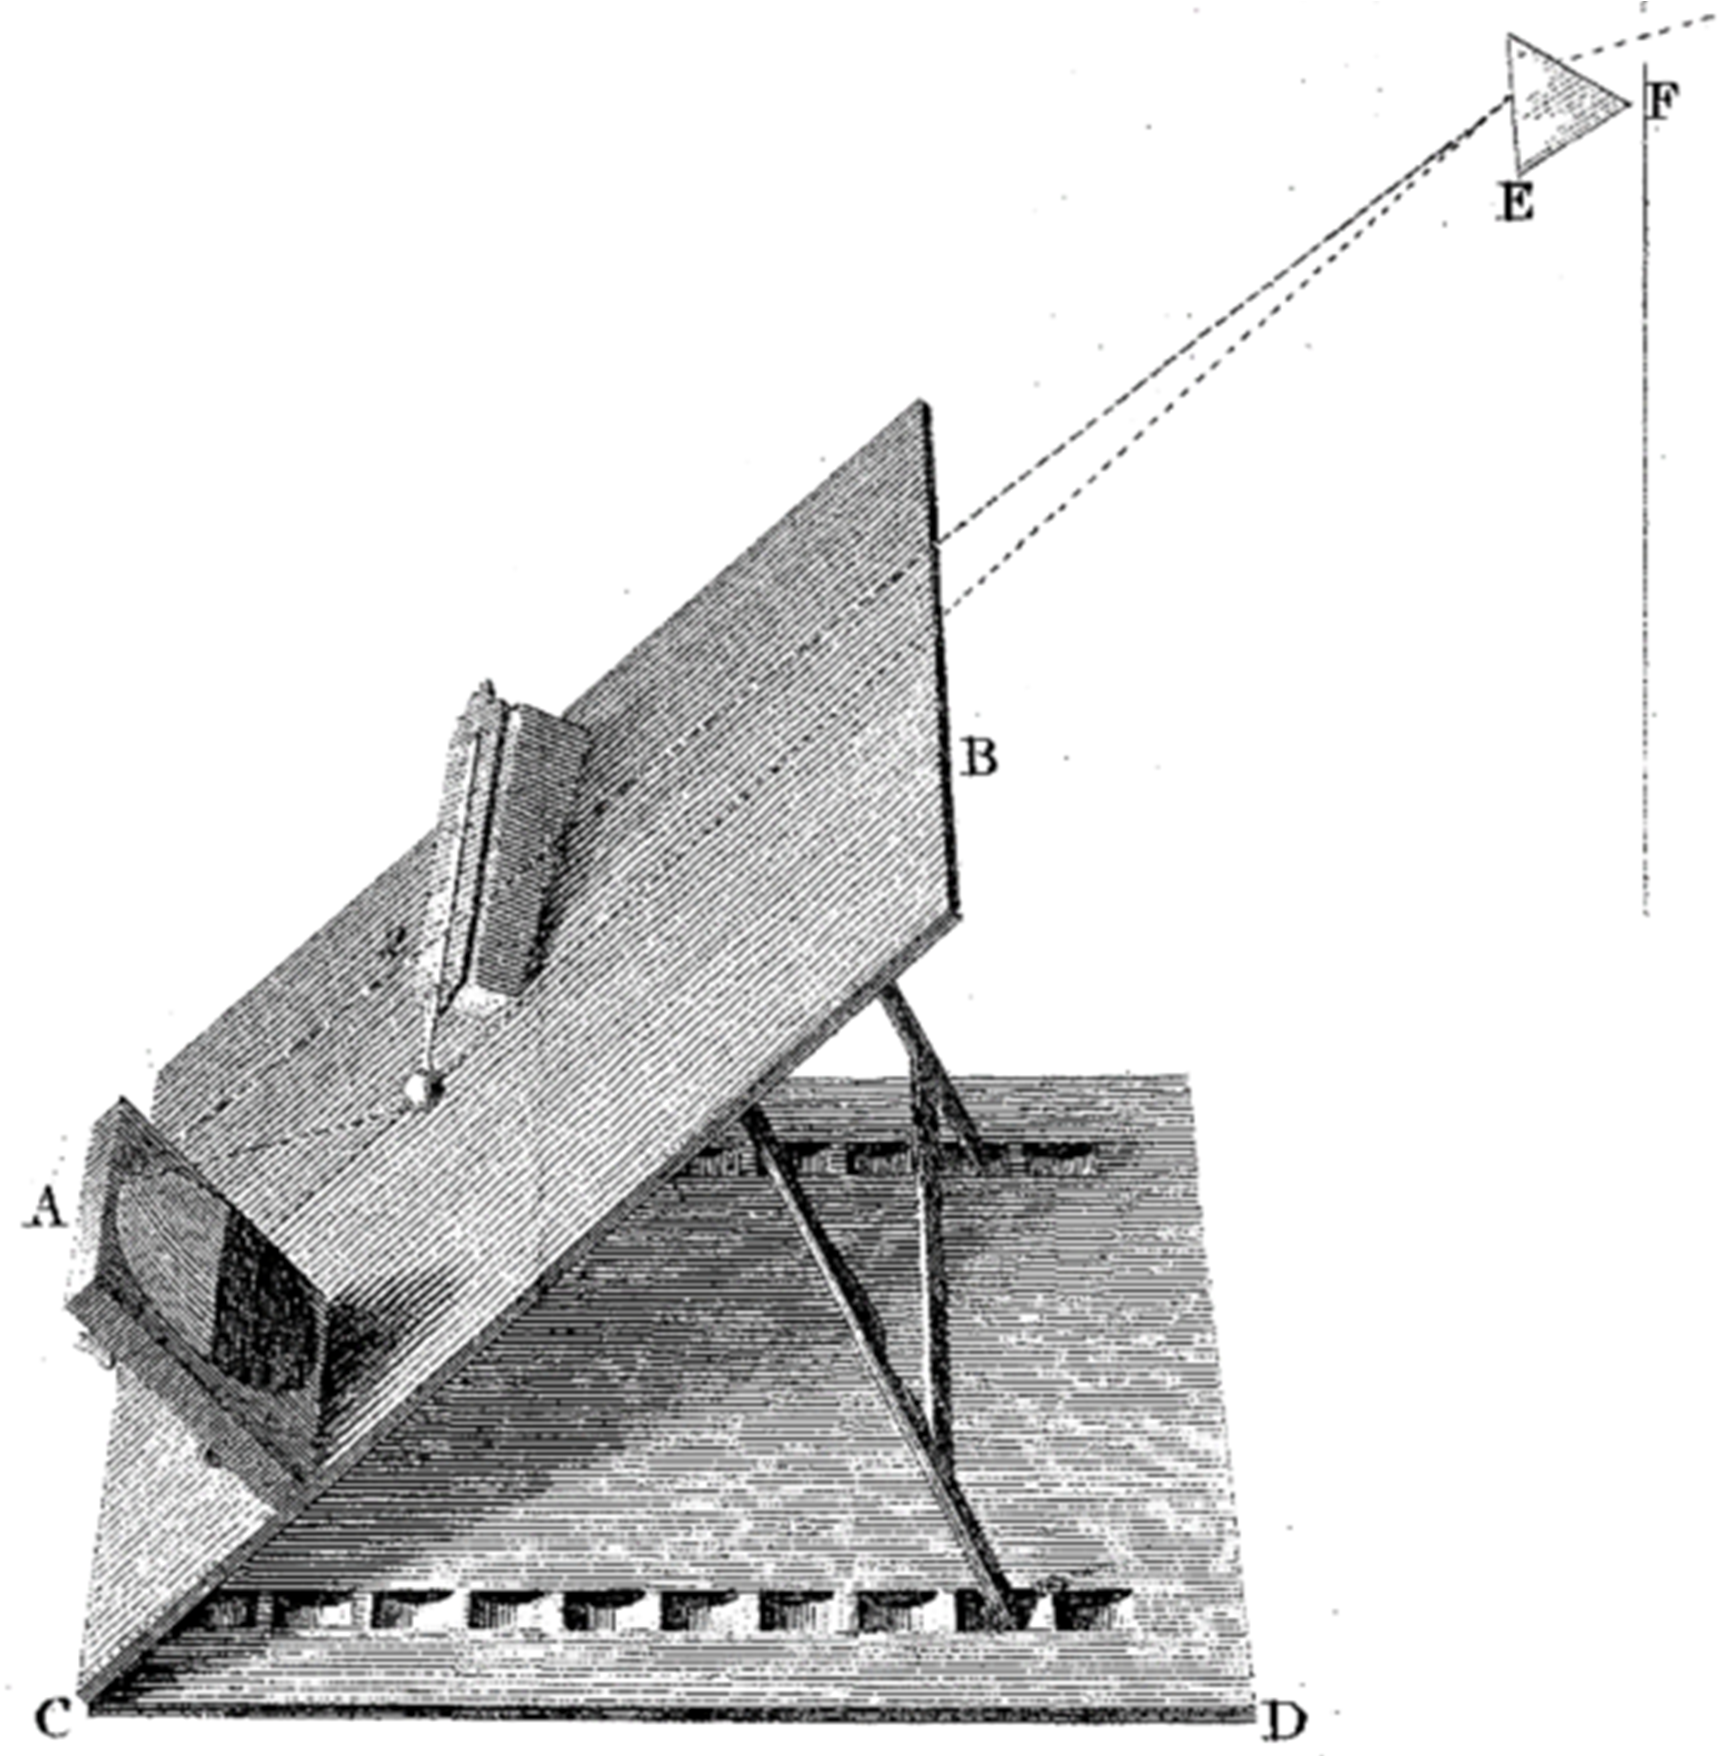
\includegraphics{figs/fundamentals/herschel_decomposition.png}
	\caption{Measurement stand for reading temperature from radiation with a single thermometer \cite{minkina_how_2021}.}
	\label{fig:herschel_decomposition}
\end{marginfigure}
\begin{marginfigure}[7cm]
	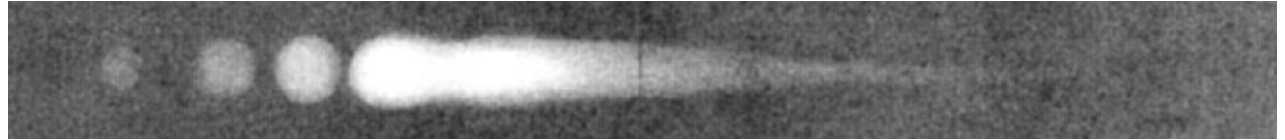
\includegraphics{figs/fundamentals/infrared_absorption.png}
	\caption{Example of thermogram originated from a wet piece of paper and targetted radiation.}
	\label{fig:infrared_absorption}
\end{marginfigure}
\begin{kaobox}[frametitle=Discovery of infrared radiation]
Heat was initially believed to only transfer through matter until the experiments of William Herschel led to the discovery of 'calorific' or 'invisible' rays. This term referred to wavelengths that fall beyond the red end and thus are invisible to the naked eye. Circa 1737, Châtelet suggested that different colours could carry different temperatures, though it would not be until 1800 that this theory was proved. W. Herschel passed the Sun's radiation through a prism and placed mercury thermometers over the split spectrum. The measured temperatures not only differed from atmospheric temperature but also the readings beyond the red end were higher. A more advanced set-up of this experiment is shown in Figure \ref{fig:herschel_decomposition}, with a reflective mirror and a platform with that can vary its slope \cite{ring_discovery_2000, minkina_how_2021, minkina_infrared_2009}. Later in 1804, John Leslie checked the discrepancies in the temperature readings of different materials, using the so-called Leslie cube. Another curious experiment showed that there exist atmospheric windows with a higher transmission factor and less absorption. W. Herschel's son, John Herschel, used the technique called evaporography to create a thermal image, also known as a thermogram, over a wet piece of paper. The result is shown in Figure \ref{fig:infrared_absorption}, with white dots representing beyond infrared wavelengths. 
\end{kaobox}

IR radiation is physically represented as electromagnetic (EM) waves that propagate through space as a sinusoidal function ($f(x) = k \cdot \sin{x}$) with a spatial periodicity, known as wavelength (\si{\meter}), $\lambda$, and a period of oscillation (\si{\second}), $\mathcal{T}$. The speed of propagation depends on the kind of wave and is calculated with the frequency $\nu$ derived from $\mathcal{T}$ and $\lambda$. However, EM waves are known to propagate at the speed of light ($c = 300 000\si{\kilo\meter}^{-1}$) in a vacuum; otherwise, $c$ depends on the index of refraction of the medium of propagation. Waves are affected by disturbance, and according to this can be organized into longitudinal and transverse waves, with both being perpendicular. Transverse waves can oscillate in many different directions, which yields the concept of polarization and plane of polarization. The latter is defined through the direction of propagation and the disturbance. If a wave is categorized as unpolarized, then the plane of polarization can adopt all possible orientations. Regarding IR radiation, it is perturbed by electric and magnetic fields, and its polarization is expressed through the first and the direction of propagation ($x-z$ plane). Therefore, the recording of waves and IR radiation can be performed by polarizers, with a simple microscopically small conducting grid being sufficient for filtering out waves that are non-perpendicular to such a grid \cite{vollmer_infrared_2017}. In thermography, the captured EM radiation is referred to \textbf{thermal radiation}, emitted by bodies at a temperature over 0\si{\kelvin} (-273.15ºC). 

The radiation measured from a surface is not solely affected by such a surface, but other factors intervene in the acquisition. Among these, the most notable factors are the absorption and scattering phenomena from atmospheric particles and sensor components, as well as the radiation emitted by surrounding objects and the atmosphere. The degree of transmissivity of the atmosphere, which may vary throughout time, is known as the transmission factor. Other minor influencing factors are the distance to the sensor, the object's emissivity, dimensions and shape, the atmospheric temperature and humidity as well as the temperature of optics \cite{vollmer_infrared_2017}. 

Although the IR spectrum covers a wide range of wavelengths (see Figure \ref{fig:introduction_scheme}), IR imaging is focused on a small part of these. Three spectral ranges are the most frequent in thermography: short-wave infrared (SWIR: 900-1700\si{\nano\meter}), mid-wave infrared (MWIR: 3000-5000\si{\nano\meter}) and long-wave infrared (LWIR: 8000-14000\si{\nano\meter}) \cite{gade_thermal_2014, vollmer_infrared_2017}. Commercial sensors are available on the three spectral ranges; whether one of them ought to be used over another must attend to criteria such as atmospheric transmission, expected radiation and the physics of detectors. A simple Scopus search shows that MWIR imaging is the most widespread, though it is significantly downgraded over SWIR and LWIR for UAS platforms (see Figure ). In this dissertation, the integrated thermographic camera operates over the LW range. 

Preferences on the LW range over SWIR and MWIR are not a casualty, but it is rather influenced by atmospheric transmissivity. Most of Earth's surface has its emission peak in this interval, while the LW range is also known as an atmospheric window where absorption is considerably smaller \cite{gonzalez_thermal_2019, quattrochi_thermal_1999}. 

An exhaustive, though not complete, list of the most frequent commercial IR cameras used for research is shown in Table \ref{table:thermographic_devices}. Every single of them is designed for measuring LWIR, while their focal length is typically over 13\si{\milli\meter}. Instead of widening the camera view, these devices acquire images focused on very specific areas with a very small image resolution. Therefore, the mentioned drawbacks ought to be considered to make an appropriate flight plan. For instance, side overlapping among different sweeps from the planned trajectory must be large enough to guarantee there exists overlapping between thermal imagery. 

\renewcommand{\arraystretch}{1.2}
\begin{table*}[h!]
    \caption{Consumer-grade thermal devices found in the literature and their specifications, according to the manufacturer's source.}
    \label{table:thermographic_devices}
    \begin{tabular}{llllll}
        \toprule
        Thermographic tool & Focal length & FOV & Image res. & Spectral range & Ref. work \\
        \midrule
        \multicolumn{6}{c}{DJI}\\
        \multirow{2}{*}{Zenmuse XT2}    & 13 \si{\milli\meter}   & $32^{\circ} \times 26^{\circ}$  & $640 \times 512$ px  & \multirow{2}{*}{LWIR (7.5 - 13.5 \si{\micro\meter})}    & \multirow{2}{*}{\cite{lopez_optimized_2021, yuan_uav-based_2021, jo_dense_2021}}\\
        & 19 \si{\milli\meter}   & $25^{\circ} \times 19^{\circ}$  & $336 \times 256$ px  &   & \\
        Zenmuse H20T     & 13.5 \si{\milli\meter}   & $31.7^{\circ} \times 25.36^{\circ}$  & $640 \times 512$ px  & LWIR (8 - 14 \si{\micro\meter})    & \cite{paziewska_integration_2022, jiang_diurnal_2022}\\
        \cmidrule{1-6}
        \multicolumn{6}{c}{FLIR}\\
        FLIR A320     & 18 \si{\milli\meter}   & $25^{\circ} \times 18.8^{\circ}$  & $320 \times 240$ px  & LWIR (7.5 - 13.5 \si{\micro\meter})    & \cite{guilbert_fusion_2020}\\
        FLIR A35     & 9 \si{\milli\meter}   & $48^{\circ} \times 39^{\circ}$  & $320 \times 256$ px  & LWIR (7.5 - 13.5 \si{\micro\meter})    & \cite{comba_2d_2019}\\
        FLIR One     & 15 \si{\centi\meter}   & $50^{\circ} \times 38^{\circ}$  & $80 \times 60$ px  & LWIR (8 - 14 \si{\micro\meter})    & \cite{javadnejad_photogrammetric_2020}\\
        FLIR A65     & 25 \si{\milli\meter}   & $25^{\circ} \times 20^{\circ}$  & $640 \times 512$ px  & LWIR (7.5 - 13.5 \si{\micro\meter})    & \cite{adan_fusion_2017, jarzabek-rychard_supervised_2020, lin_fusion_2019, westfeld_generation_2015}\\
        FLIR Tau2 640     & 13 \si{\milli\meter}   & $45^{\circ} \times 37^{\circ}$  & $640 \times 512$ px  & LWIR (7.5 - 13.5 \si{\micro\meter})    & \cite{boesch_thermal_2017, sledz_thermal_2018}\\
        \cmidrule{1-6}
        \multicolumn{6}{c}{Sensefly}\\
        Sensefly thermoMAP     & N.A.   & N.A.  & $640 \times 512$ px  & LWIR (7.5 - 13.5 \si{\micro\meter})    & \cite{padua_vineyard_2019}\\
        \bottomrule
    \end{tabular}
\end{table*}
\renewcommand{\arraystretch}{1}

\subsubsection{Hyperspectral imaging}

Hyperspectral imaging (HSI) differs from multispectral imaging in the number of bands, wavelengths and bandwidth of these. Hyperspectral images are 3D data cubes known as \textbf{hypercubes}, where each pixel is defined within a continuous spectrum range. The spectral resolution is typically given in \si{\nano\meter} or as a number of bands, though the first is preferred as the resolution can vary throughout the covered interval. Spectral signatures are complete and differentiable over the observed wavelength range, and thus, hypercubes outperform discrete multispectral data on the classification, segmentation and unmixing of materials. For instance, different varieties of plants might have a radiative response too similar among them, even using HSI. Therefore, IA algorithms could be applied to the automatic detection of the most discriminative wavelengths and be accordingly weighted to provide a meaningful result from input data. 

Unlike other imaging tools, HSI has undergone a rising path from major to minor; from satellite scanning to UAV and laboratory applications. Hence, it is applied in a wide range of applications, from phenotyping, cultural heritage, medical research and food processing to biochemistry and the monitoring of Earth's processes and areas of interest, among others \cite{amigo_hyperspectral_2019, }. Also in contrast to multispectral imaging, preprocessing on HSI has been significantly treated in the literature until recently. Remotely sensed data is affected by several factors, including acquisition conditions and random errors caused by sensors as well as atmospheric and surface effects. 

\lstinputlisting[language=python, caption={Function for finding the most similar wavelength among those available for a specific sensor data.}, label=code:nearestband]{code/nearest_band.py}

Radiometric correction over HSI has been conducted to obtain representative data from Earth's surfaces. The bibliography on this field has covered many topics, though it is mainly focused on satellite imaging. While some of the studied techniques can be applied to UAV imaging, other chapters are irrelevant to our target platforms, UAVs. For instance, atmospheric effects such as absorption are of no interest in close-range work. However, the low flight altitude, the UAV instability or its viewing angle harden the pre-processing operations \cite{jakob_need_2017}. Geometric and radiometric corrections as well as spectral calibrations are also required to obtain accurate data \cite{adao_hyperspectral_2017}. Geometric distortions refer to those defects caused primarily by the UAV instability as well as due to the acquisition technique. For instance, push-broom sensors present higher geometric distortions that can be reduced by means of stabilizers. Geometric correction can be achieved with an INS, GPS and Digital Elevation Model (DEM). Although there exists commercial software based on this approach, it requires a high-precision system for accurate correction. Instead, GCPs have been extensively used to ensure correct positioning \cite{ramirez-paredes_low-altitude_2016}. Also, the dual acquisition of visible and hyperspectral imagery allows matching both data sources \cite{jurado_efficient_2021, xue_compact_2021, ramirez-paredes_low-altitude_2016}, with the visible data being geometrically correct. Alternatively, feature matching among overlapping images has also been shown to help with geometric correction \cite{akhoundi_khezrabad_new_2022}.

Similarly to geometric distortions, radiometric defects can be corrected with software tools from the hyperspectral manufacturer. The objective is to transform the sensor's DNs to radiance, influenced by acquisition conditions, and reflectance of Earth's surfaces, regardless of previous conditions. Thus, the second result must be applied to Deep Learning techniques for their application over any hyperspectral dataset. To this end, the coefficients needed for this correction are typically calibrated in the laboratory. However, they are more likely to vary through time \cite{adao_hyperspectral_2017}, thus leading to worsening the radiometric correction. This process can be supported by the use of grayscale tarps whose reflectance is known, thereby allowing to perform linear interpolations to calibrate the acquired DN \cite{lucieer_hyperuasimaging_2014} with the empirical line method (ELM) \cite{aasen_quantitative_2018, sousa_uav-based_2022}. Dark and grey/white references are required to perform this linear interpolation\cite{jakob_need_2017, sagan_data-driven_2022, duan_land_2013}, typically from isotropic materials (near to Lambertian) that present a grayscale palette. Alternatively, the acquisition of radiance samples can help to transform DNs with fitting methods such as the least-square method (LSM). Sensor-based factors, including the vignetting effect that causes a drop in the intensity, lead to a different radiometric response in pixels of the same bands \cite{yang_dom_2017}.

Atmospheric corrections have also been documented for UAV flights. Accordingly, the at-sensor radiance can be correlated to the surface hemispherical-directional reflectance function (HDRF) measured in the laboratory beforehand. The previously grayscale palette in Lambertian materials can be used to achieve this \cite{lucieer_hyperuasimaging_2014}. Physically-based methods have also been investigated by measuring the atmospheric conditions that conditioned the hyperspectral imaging, though they are more time-consuming. Finally, some public repositories offer atmospherically corrected datasets, e.g., the Aviris data portal \cite{california_institute_of_technology_aviris_nodate}, whereas widely known software for hyperspectral processing also includes semi-automatic correction algorithms (ENVI, Headwall SpectralView, etc). Other studies calculate the Bidirectional Reflectance Distribution Function (BRDF) of visible materials. Previous corrections are applied, and BRDF kernels are estimated using kernels such as Ross and Li from the varying response of materials according to solar and view angles \cite{queally_flexbrdf_2022, jia_kernel-driven_2020, sagan_data-driven_2022}.

The list of hyperspectral sensors on the market that can be coupled with UAVs has significantly increased in recent years. Therefore, Table \ref{table:hyperspectral_devices} solely illustrates those that provide higher spectral resolution and have been explored in the hyperspectral state-of-the-art literature. As previously regarded, the spectral range can be calculated from the spectral resolution, in \si{\nano\meter}, and the number of bands. However, as observed in Table \ref{table:hyperspectral_devices}, this is not exactly right for every sensor as the spectral resolution may not be constant. In this dissertation, the research focused on hyperspectral imaging operates over data cubes from Headwall Photonics Inc.\textregistered Nano HyperSpec with  sampling intervals ranging from 2.2\si{\nano\meter} to 6\si{\nano\meter} in the central wavelengths.

\renewcommand{\arraystretch}{1.2}
\begin{table*}[h!]
    \caption{Consumer-grade thermal devices found in the literature and their specifications, according to the manufacturer's source.}
    \label{table:hyperspectral_devices}
    \begin{tabular}{lllllll}
        \toprule
        Tool & Spectral range & \#Bands & Spectral res. & Acquisition & Spatial res. & Ref. work \\
        \midrule
        \multicolumn{7}{c}{Headwall Photonics}\\
        Nano HyperSpec & 400-1000\si{\nano\meter}   & 272-775 & 6\si{\nano\meter}  & Push-broom    & 640 px  &\cite{sankey_uav_2018, sousa_uav-based_2022}\\
        Micro Hyperspec & 400-1000\si{\nano\meter}   & 837-923 & 2.5\si{\nano\meter}  & Push-broom    & 1004 px  &\cite{sousa_uav-based_2022}\\
        \cmidrule{1-7}
        \multicolumn{7}{c}{SENOP}\\
        VIS-VNIR Snapshot & 400-900\si{\nano\meter}   & 380 & 10\si{\nano\meter}  & Snapshot    & $1010\times1010$ px & \cite{sousa_uav-based_2022}\\
        HSC-2 & 450-900\si{\nano\meter}   & Up to 1000 & 6-18\si{\nano\meter}  & Snapshot    & $1024\times1024$ px & \cite{sousa_uav-based_2022}\\
        \cmidrule{1-7}
        \multicolumn{7}{c}{XIMEA}\\
        XIMEA SNm4x4 & 460-600\si{\nano\meter}   & 16 & 15\si{\nano\meter}  & Snapshot    & $512\times272$ px & \cite{gao_cbff-net_2023}\\
        \cmidrule{1-7}
        \multicolumn{7}{c}{Specim}\\
        AISA Angle & 400-970\si{\nano\meter}   & 488 & 2.9\si{\nano\meter}  & Pushbroom    & $1024$ px & \cite{windrim_unsupervised_2023}\\
        FX17 & 900-1700\si{\nano\meter}   & 224 & 8\si{\nano\meter}  & Pushbroom    & $640$ px & \cite{sousa_uav-based_2022}\\
        \cmidrule{1-7}
        \multicolumn{7}{c}{Cubert GmbH}\\
        UHD 185 Firefly & 450-950\si{\nano\meter}   & 125 & 8\si{\nano\meter}  & Snapshot    & $1000\times1000$ px & \cite{yue_comparison_2018}\\
        \bottomrule
    \end{tabular}
\end{table*}
\renewcommand{\arraystretch}{1}

\subsection{Active sensing}

Active systems, unlike previous passive sensors, provide their own energy source and therefore do not rely on external light sources, radiation emitted and reflected by surfaces and weather conditions \cite{dong_lidar_2018}. Among active sensors, the focus of this dissertation is on Light Detection and Ranging (LiDAR). It is an optical remote sensing technique that measures the properties of scattered light and can be used on spaceborne, airborne and ground-based platforms. The emitted energy is bounced back after colliding on Earth's surfaces, thus being capable of determining distances by measuring the time delay between emission and reception. It is also aimed at measuring speed (wind LiDAR) and attenuation of volume targets such as the atmosphere or seawater \cite{emery_introduction_2017}. The emitted electromagnetic energy operates at a wavelength, with LiDAR working at much shorter wavelengths than RADAR, typically in atmospheric transmission windows. Some of these were previously reviewed (infrared), although LiDAR systems also operate at the visible and ultraviolet (UV) spectral range. This parameter determines which is the minimum size of objects to be detected, with shorter wavelengths being more sensitive to smaller particles. Hence, LiDAR systems are typically used for atmospheric and meteorology research. Backscattering is dependent on the dielectric discontinuity produced by collided surfaces, and therefore, nonmetallic objects have significantly lower responses to higher wavelengths \cite{dong_lidar_2018}. 

A simplification of LiDAR emissions is the concept of ray: $r(t) = o + \vec{d}t$. This is a geometric data type defined by the starting position, $o$, and a direction vector, $\vec{d}$, that infinitely spread in the space. Unlike rays in CG, LiDARs emit volumetric beams whose targets are surface areas rather than points. Therefore, impacts on surfaces may not entirely block these beams, thus leading to penetrating surfaces that harden the visualization of objects below it but are not completely enclosed. For example, LiDAR has been applied to archaeology with notable results since it allows removing points from high-density forests and uncovers remains at the Earth's surface. Other widespread applications of LiDAR technology are in \gls{Remote sensing}, geology, atmospheric physics or seismology \cite{emery_introduction_2017}. More specific ones concerning our work are building inspections \cite{shariq_revolutionising_2020}, monitoring of natural environments (landform dynamics \cite{guisado-pintado_3d_2019}, ecological resilience \cite{mitasova_geospatial_2010}, etc.), autonomous driving \cite{kuutti_survey_2021}, preservation of cultural heritage \cite{andriasyan_point_2020}, land mapping or urban planning \cite{zhou_street-view_2022}.

Similar to previous optical sensors, LiDAR sensors are also influenced by factors such as the local incidence angle between the surface normal and the radar beams, $\gamma$, and the dielectric properties of materials, expressed as $\varepsilon = \varepsilon' + j\varepsilon''$, with the dielectric constant depending on the permittivity ($\varepsilon'$) and the loss factor (the imaginary part, $\varepsilon''$). Other major factors are polarization, i.e., the orientation of the transmitted electromagnetic vectors, and the surface roughness.

Most common LiDAR operates on the 600-1000\si{\nano\meter} spectral range for non-scientific applications; ground-based are frequently in 500-600\si{\nano\meter}, whereas airborne systems work over 1000-1600\si{\nano\meter}. The second is of special interest for this dissertation and thus we will stick to it. Despite being more expensive, these are also eye-safe due to working at larger wavelengths. Nevertheless, most of commercial sensors operating below 1000\si{\nano\meter} are eye-safe nowadays. Airborne LiDAR can record several discrete measurements per emitted pulse, or record a signal sampled with a frequency determined by time interval or distance (for example, sampled every 1\si{\nano\second} or 15\si{\centi\meter}). The latter is known as full-waveform LiDAR and is mainly used in forestry applications since it provides a signature that helps on estimating the density at different height levels. On the other hand, discrete-return LiDAR has found a wider number of applications. A minimal operative LiDAR is composed of laser and receiver units, GPS and IMU systems and control, monitoring and recording units. Hence, one of the main shortcomings of imagery is overcome by LiDAR, as recorded 3D points are georeferenced. 
\begin{gather}
    \label{eq:lidar_distance}
    \begin{aligned}
        R &= \frac{1}{2}ct_s
    \end{aligned}
\end{gather}

Equations \ref{eq:lidar_distance} and \ref{eq:lidar_equation} may shed some light on the functioning of LiDAR systems. First, the distance of the surface that returned the backscattered energy, $R$, is calculated according to the time delay, $t_s$, and the speed of light, $c$. Also, the acquired energy, involving both emitter and receiver, is expressed as shown in Equation \ref{eq:lidar_equation}. There are multiple formulae in the literature to represent how is LiDAR intensity retrieved, though of most them are analogous \cite{hofle_correction_2007, bolkas_effect_2018, dong_lidar_2018}.
\begin{gather}
    \label{eq:lidar_equation}
    \begin{aligned}
        \sigma &= \frac{4\pi f_{r}(\vec{w})A_{t}}{\Omega}\\
        A_{t} &= \frac{\pi R^{2} \beta^{2}_{t}}{4}\\
        P_{r} &= \frac{\bar{I} D^{2}_{r} \eta_{atm} \eta_{sys} \sigma}{4 \pi R^{4}}=
        \frac{4\pi^2 \bar{I} D^{2}_{r} \eta_{atm} \eta_{sys}  f_{r}(\vec{w})}{4\Omega R^{2} \beta^{2}_{t}}
    \end{aligned}
\end{gather}
where $\bar{I}$ is the emitted energy, $D^{2}_{r}$ is the receiver diameter (\si{\meter}), $\eta_{atm}, \eta_{sys}$ are atmospheric and system transmission factors, $f_{r}(\vec{w})$ is the target reflectance, $A_{t}$ is the target area, $R$ is the distance to receiver in \si{\meter}, $\beta$ is the transmit beam width (\si{\radian}) and $\Omega$ is the scattering solid angle (\si{\steradian}). Again, $\pi$ appears as a division factor than controls the amount of energy spreading a specific point. Instead, the emission energy spreads in every possible direction within a semisphere.

Lasers are the main unit in LiDAR systems, and energy emitted by these can be oriented through a scan deflector. If orientation of lasers vary, so does the scanning pattern. The fundamental deflections are based on polygonal mirroring, which generates parallel scan lines and swinging mirrors with zig-zag patterns, thus achieving more point density at the line boundaries. Other deflections are fibre-optics, which produces a similar output to polygonal mirroring despite changing beam transmission technology, and rotating slanted mirrors that generate elliptical shapes. Finally, Risley prism scanners such as DJI Livox have a different pattern for sampling surfaces with more density and longer integration times.

\begin{figure*}[!ht]
	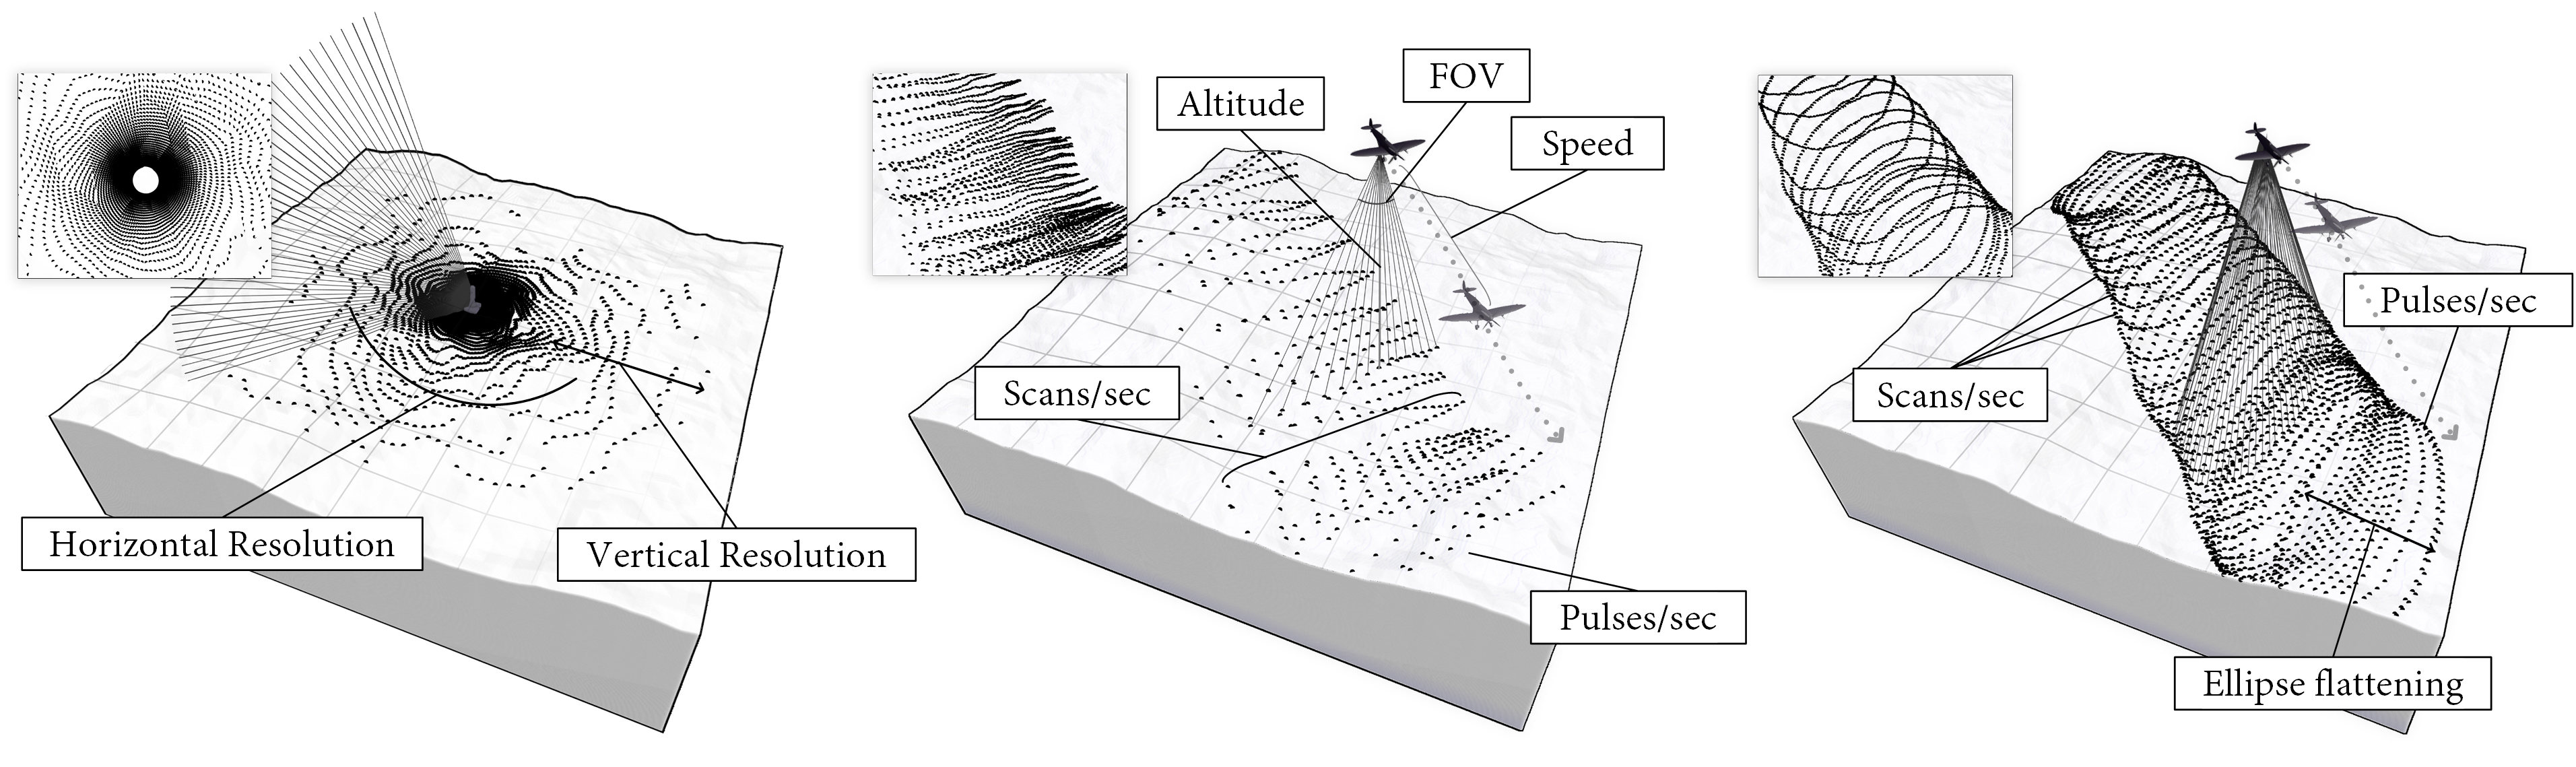
\includegraphics[width=\linewidth]{figs/fundamentals/lidar_patterns.png}
	\caption{Surveys performed with different path planning: a) the path is automatically computed according to the sensor's FOV, whereas in b) the path is drawn by the user, simplified using the Douglas-Peucker algorithm and subsampled using a Catmull-Rom spline. Zoomed-in images at the top-right corner show the effect of jittering. }
    \label{fig:lidar_patterns}
\end{figure*}

Table \ref{table:lidar_devices} shows a brief list of some widespread LiDAR sensors, both land-based and airborne. It provides further insight into which are the most frequent wavelengths. Among these, LiDAR sensors operating at 532\si{\nano\meter} are also known as bathymetric and enable capturing shallow, underwater surfaces. Thus, it is especially relevant for hydrology and coastal monitoring.

\renewcommand{\arraystretch}{1.2}
\begin{table*}[h!]
    \caption{Most common LiDAR systems in the literature and their attributes.}
    \label{table:lidar_devices}
    \begin{tabular}{lllllll}
        \toprule
        LiDAR system & FOV & Echoes & Maximum range & Wavelength & Channels & Points/\si{\sec} \\
        \midrule
        \multicolumn{7}{c}{Velodyne}\\
        HDL-32E    & $360^{\circ}\times41.3^{\circ}$    & 2   & 80-100\si{\meter} & 903\si{\nano\meter} & 32 & 1.39M\\
        Puck/Puck LITE    & $360^{\circ}\times30^{\circ}$    & 2   & 100\si{\meter} & 903\si{\nano\meter} & 16 & 600K\\
        Puck Hi-RES    & $360^{\circ}\times20^{\circ}$    & 2   & 100\si{\meter} & 903\si{\nano\meter} & 16 & 600K\\
        ULTRA Puck    & $360^{\circ}\times40^{\circ}$    & 2   & 100\si{\meter} & 903\si{\nano\meter} & 32 & 1.2M\\
        Alpha Prime    & $360^{\circ}\times40^{\circ}$    & 2   & 250\si{\meter} & 903\si{\nano\meter} & 128 & 4.8M\\
        \cmidrule{1-7}
        \multicolumn{7}{c}{Valeo}\\
        SCALA Gen 2    & $133^{\circ}\times10^{\circ}$    & 3   & 200\si{\meter} & 905\si{\nano\meter} & 16 & 25\si{\hertz}\\
        \cmidrule{1-7}
        \multicolumn{7}{c}{SICK}\\
        MRS1104C-111011    & $275^{\circ}\times7.5^{\circ}$    & 3   & 64\si{\meter} & 850\si{\nano\meter} & 32 & 165K\\
        \cmidrule{1-7}
        \multicolumn{7}{c}{Phoenix Systems}\\
        SCOUT-M2X   & $360^{\circ}\times40.3^{\circ}$    & 3  & 300\si{\meter} & 905\si{\nano\meter} & 32 & 640K\\
        SCOUT-32   & $360^{\circ}\times40^{\circ}$    & 2  & 220\si{\meter} & 905\si{\nano\meter} & 32 & 600K\\
        HydroRANGER   & $40^{\circ}$ VFOV  & 15  & 75\si{\meter} & 532\si{\nano\meter} & - & 200K\\
        RANGER-LR LITE   & $360^{\circ}$ HFOV  & 5  & 1000\si{\meter} & 1550\si{\nano\meter} & - & 1.5M\\
        \bottomrule
    \end{tabular}
\end{table*}
\renewcommand{\arraystretch}{1}

\subsection{Principles of physical measurement}

\gls{Remote sensing} covers a wide range of spectral wavelengths, making images that show the emitted and reflected radiation from the Earth's surfaces, including matter such as atmospheric particles and bare soil. A huge number of conditions and parameters are involved in the observed radiation, whose explanation would cover dozens of pages, if not a book. Hence, only a few remarks will be done here. 

A key ingredient in the understanding of the scene is the detailed specification of the appearance of materials regardless of light and the influence of other matter. Energy, as captured in nature, does not depict the underlying appearance of materials but the appearance when some specific circumstances are met. Therefore, measurements ought to be processed to make them independent from environmental and light conditions as well as surrounding surfaces. Not only it helps in the classification of materials present in the scene, given reference spectral signatures, but also enables simulating lighting as occurs in real-world scenarios. For the latter, surfaces are assigned a spectral appearance that will not be rendered as so and thus will undergo changes as light and other matter interfere. 

Vollmer and Mollmann \cite{vollmer_infrared_2017} provided an exhaustive list of parameters conditioning the material emissivity, regardless of surrounding objects. Materials are the most differentiating feature, naïvely split into metal and nonmetal, where the latter are frequently returning higher emissivity. Also, the roughness level affects the outcome considerably; polished surfaces have lower emissivity and the contrary happens for rough surfaces. Further insight into energy dispersion helps to understand that it does not propagate over every direction of a semisphere with the same strength. Unlike blackbodies, which behave as perfect isotropic emitters, materials vary the emitted radiation conditioned to the outgoing direction. A key factor in this regard is the normal vector of the surface: the smaller the angle between the camera view direction and the normal vector, the higher the observed emissivity. However, this does not hold up for every material since conductors show the opposite behaviour. Similarly, the physical behaviour of light transport, including reflects, leads to increasing the emissivity for grooved surfaces as a consequence of rebounds. As will be observed throughout this dissertation, the spectral signature of materials is not constant, and therefore, some intervals are preferred over others in the seek of capturing a high emissivity from the target surfaces. For example, the Near Infrared (NIR) comprises the peak emissivity of vegetation. Finally, surface temperature also leads to slight emissivity changes.

\begin{figure}[!ht]
	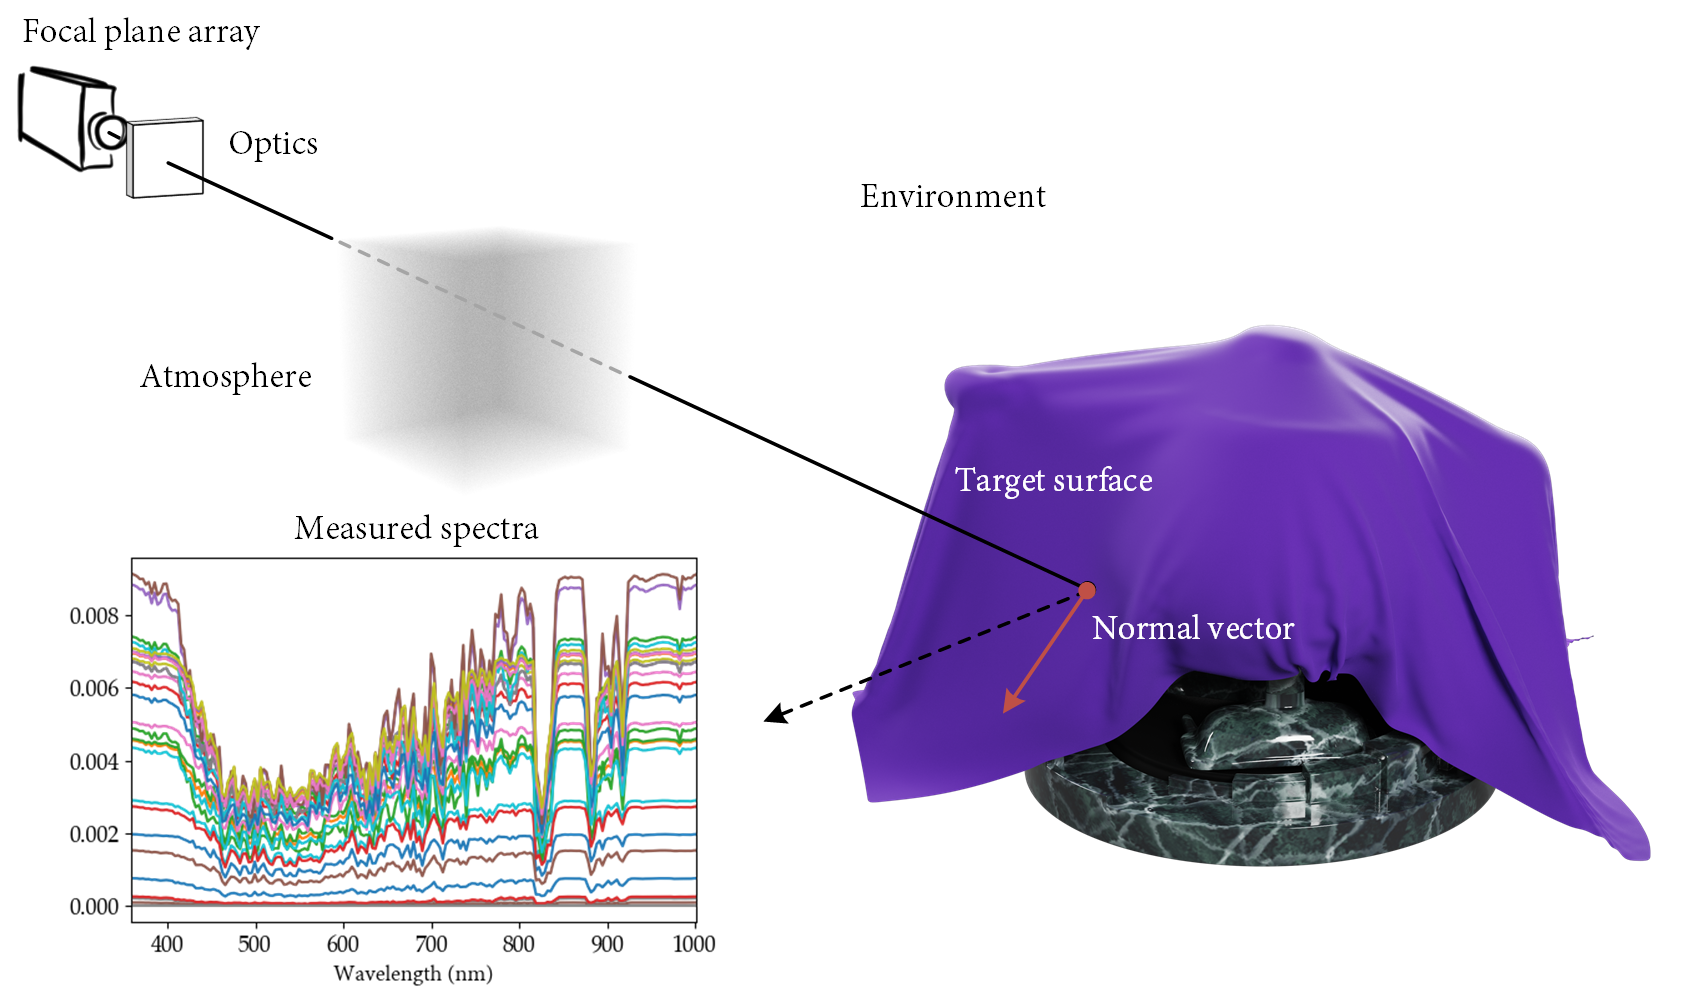
\includegraphics[width=\textwidth]{figs/fundamentals/physic_principles.png}
	\caption{Comparison of analytical BRDFS: a) Cook-Torrance ($f_0 \gets 1$, $\alpha \gets 0.077$), b) Phong ($ns \gets 32$) and c) Oren-Nayar ($\alpha \gets 0.75$). }
    \label{fig:physic_principles}
\end{figure}

\begin{marginfigure}[3cm]
	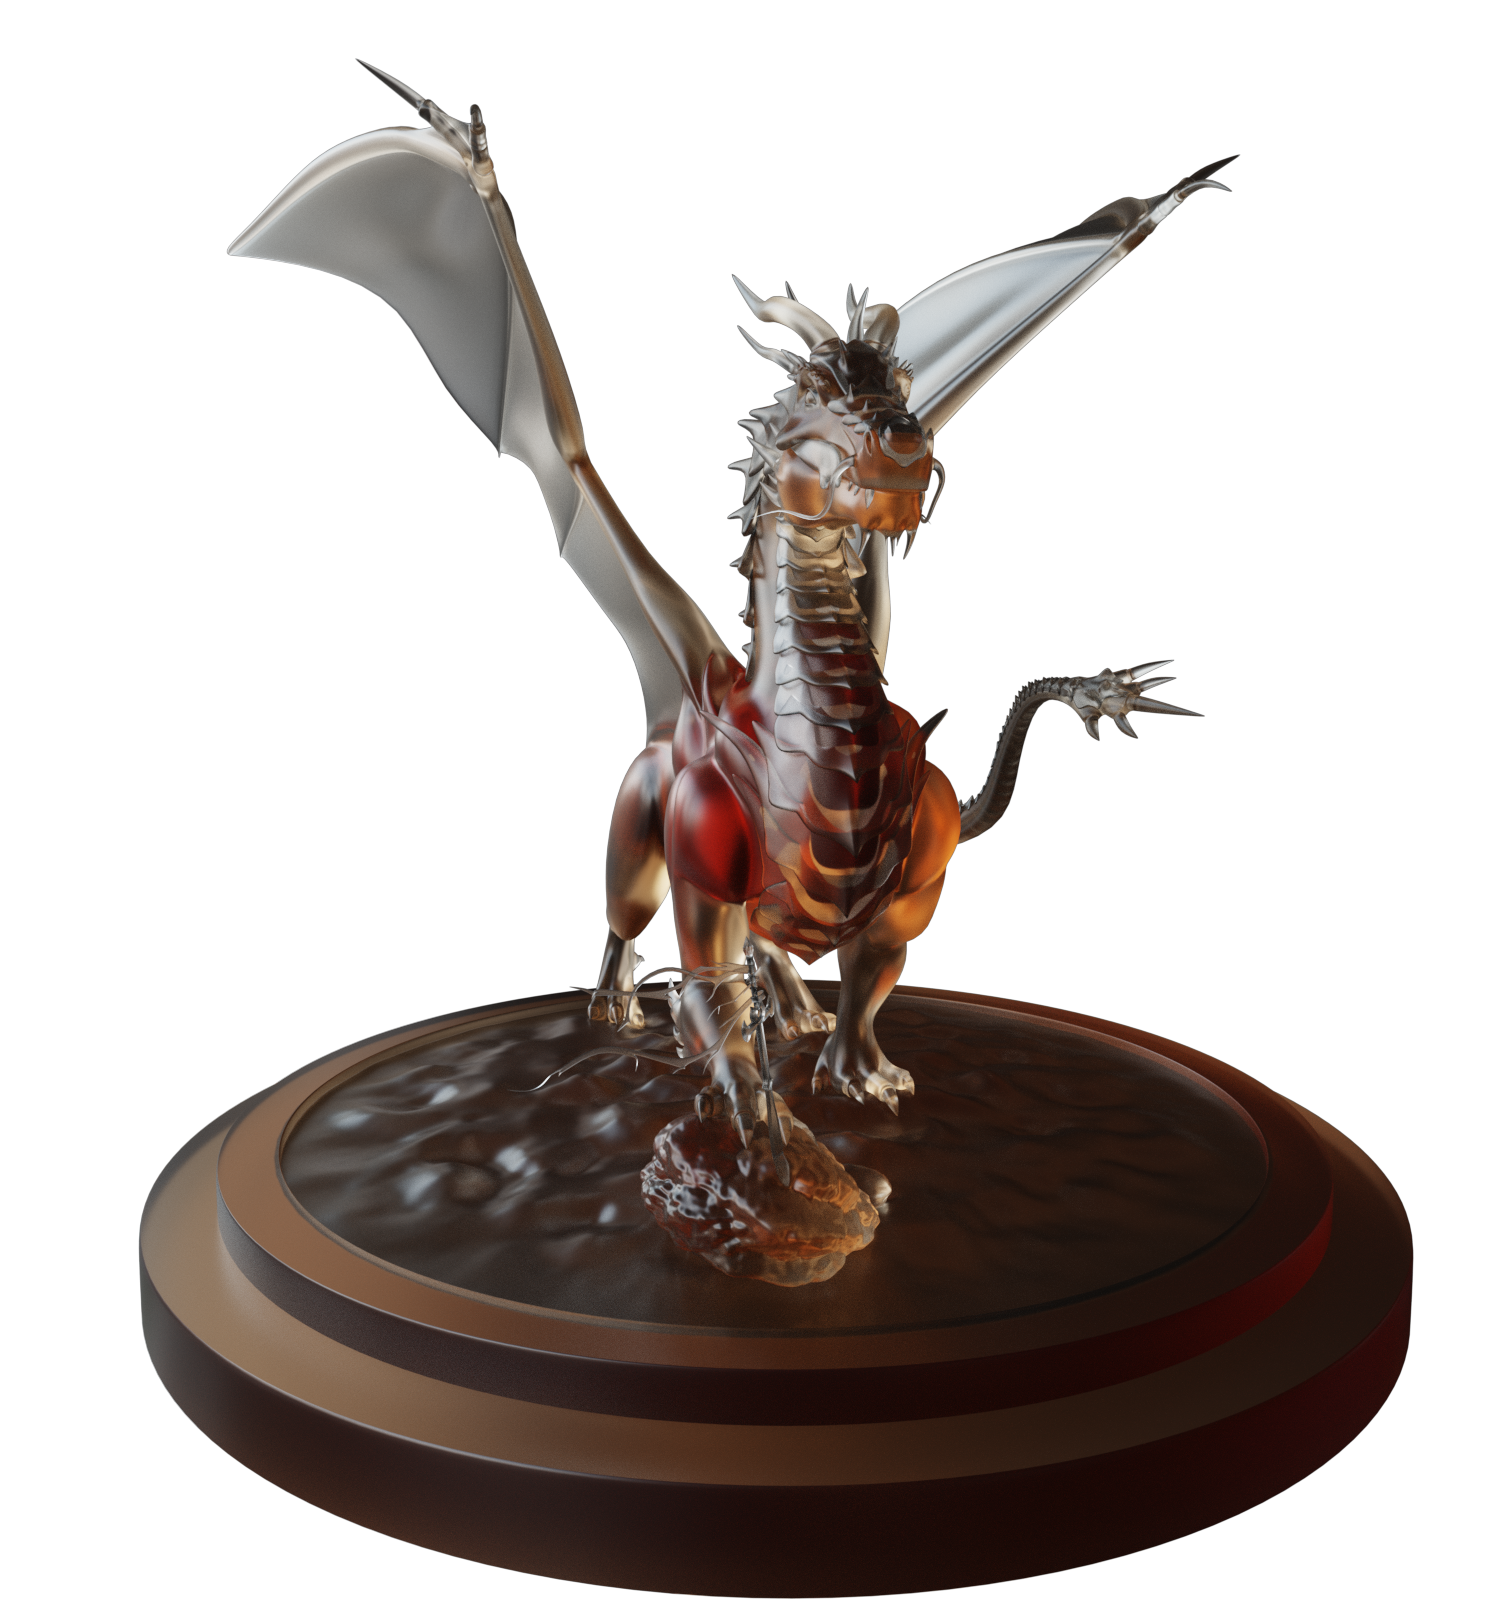
\includegraphics{figs/fundamentals/bssdf_2.png}
	\caption{Subsurface scattering simulated over a triangle mesh.}
	\label{fig:bssdf}
\end{marginfigure}
Radiometric measurements are layered data that can be carved to find the surfaces' spectral signatures. However, these corrections are simple approximations that consider a few of the mentioned factors rather than the overwhelming amount of uncontrolled attributes that can be found in nature. Otherwise, measurements can be performed with controlled surface features and lighting to provide databases of a wide range of materials \cite{dupuy_adaptive_2018}. Furthermore, databases on surface appearance comprise a number of discrete spectral signatures for each material, as these are typically parameterized by the input vector, $\omega_i$, and output direction where radiance spreads, $\omega_o$. Otherwise, these vectors can be notated as local cartesian coordinates, half-angle difference parametrization and spherical coordinates, which are also very frequent. The latter are expressed through four angles, $\varphi_i = \atan(y_i / x_i)$, $\varphi_o = \atan(y_o / x_o)$, $\theta_i = \acos(z_i)$ and $\theta_o = \acos(z_o)$. These functions, provisionally expressed as $f(\omega_i, \omega_i)$, parameterized with $\omega_i$, $\omega_o$, or their equivalent spherical coordinates, represent what was coined as Bidirectional Reflectance Distribution Functions (BRDF), or yet more intricate, Bidirectional Scatter Distribution Functions (BSDF), Bidirectional Scattering Surface Distribution Functions (BSSDF). Both BSDF and BSSDF are aimed at simulating the indirect light transport from surrounding surfaces as well as their own surfaces. BSSDF are particularly hard to calculate as the entering and exit points vary, i.e., surfaces are not opaque; instead, light travels through matter to provide a transparent-like, yet opaque, appearance. From now on, we will only refer to BRDF as the two last functions are beyond the scope of this dissertation.
\begin{marginfigure}[3cm]
	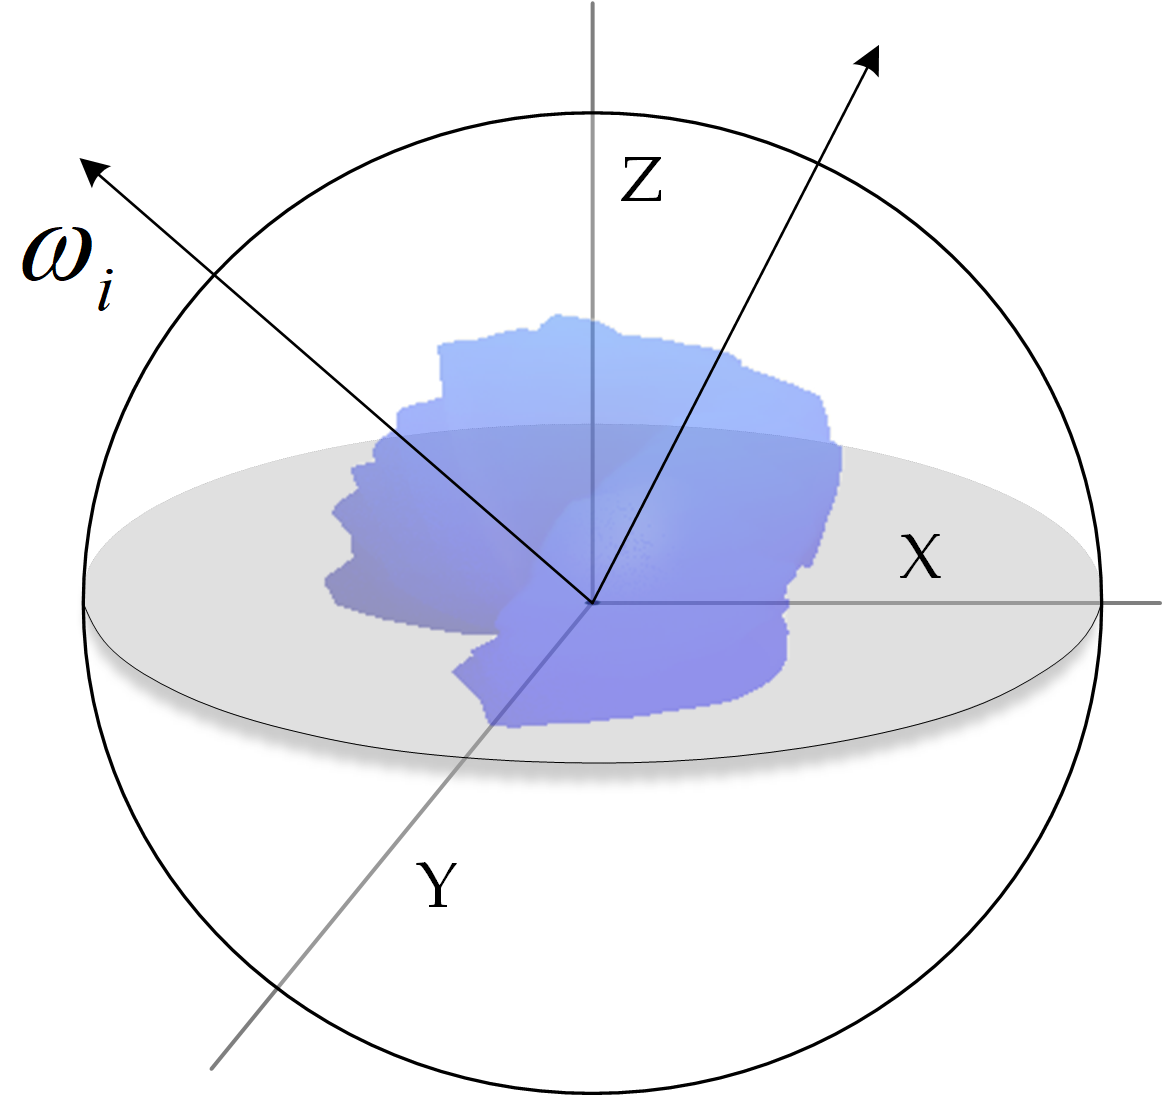
\includegraphics{figs/fundamentals/brdf_wi_wo.png}
	\caption{Parameterization of the BRDF response.}
	\label{fig:brdf_wi_wo}
\end{marginfigure}

In the last years, hyperspectral data acquisition has significantly increased, benefiting from the use of more cost-effective sensors and versatile platforms. On the one hand, traditional systems, which are deployed in the laboratory, are currently more efficient and capable of getting accurate spectral measurements of isotropic and anisotropic materials. These are gaining in accuracy, efficiency, and ease of use. At the laboratory level, the most accurate and well-known technique for collecting the optical features and BRDFs of any real-world material is the use of a goniophotometer \cite{riviere_multispectral_2012}. Different variants of this configuration have been developed either to obtain better results in anisotropic materials, to take into account refraction phenomena or even to obtain normal maps, or other characteristics that allow the sample to be modeled synthetically \cite{tunwattanapong_acquiring_2013, chen_reflectance_2014}. 

The first databases only included anisotropic materials that captured red, green and blue spectral responses as a dense set of measurements \cite{matusik_data-driven_2003}, instead of analytical functions. Thus, discretized representations are more likely to be parameterized to build larger, yet realistic, BRDF datasets \cite{serrano_intuitive_2016}. More recently, the provided wavelengths have been extended to the whole spectra available for a motorized goniophotometer, thus allowing to extend render engines beyond the visible spectra \cite{dupuy_adaptive_2018}. As a result, BRDFs are not solely parameterized through two spatial vectors, but also with a radiometric value. Hence, $f$ is now expressed as $f(\omega_i, \omega_o, \lambda)$, with $\lambda$ being the target wavelength. Accordingly, coarse radiometric resolution can be simulated as $\int_{\lambda_i}^{\lambda_j} f(\omega_i, \omega_o, \lambda) \hspace{1mm} d\lambda$. 

These advances lead us toward the generation of real-world material databases, which are highly used for rendering photorealistic scenes, virtual interior design in architecture, the game industry, etc. These applications can be enhanced by the increasing availability of real-world scenarios, which can be efficiently reconstructed using versatile platforms. However, building material databases is time-consuming, prohibitive when it comes to acquisition devices and requires considering a list of laboratory constraints. 

Due to the large measurement time, UAV flights carrying an hyperspectral sensor have been proposed for the collection of material BRDFs. These comes at expense of noisier data that must be corrected afterwards. In addition, a single or a few flights yield very incomplete spatial response due to the low variety of $\omega_o$ measurements \cite{jurado_efficient_2022}. There have been studies on atmospheric corrections for UAV flights, which involve correlating the at-sensor radiance to the surface hemispherical-directional reflectance function (HDRF) measured in the laboratory beforehand. Grayscale palettes in Lambertian materials can be used for this purpose  \cite{lucieer_hyperuasimaging_2014}. While physically-based methods have also been explored, they tend to be more time-consuming. In addition, public repositories such as the Aviris data portal (California Institute of Technology) \cite{california_institute_of_technology_aviris_nodate} offer atmospherically corrected datasets. Other widespread hyperspectral processing software, such as ENVI and Headwall SpectralView, include semi-automatic correction algorithms \cite{queally_flexbrdf_2022, jia_kernel-driven_2020, sagan_data-driven_2022}. Besides the challenging correction of samples taken from UAVs, a few studies are also aimed at finding the BRDF of visible materials. Previous corrections are applied, and BRDF are estimated using kernels such as Ross and Li from the varying response of materials according to solar and view angles \cite{queally_flexbrdf_2022}.

The lack of computational power and real-world material samples led to the Computer Graphics community approximating realistic shading with analytical functions. These are easier to solve and integrate into script-based routines such as vertex and fragment shaders. They intend to emulate the appearance of real-world materials; however, continuous functions are smoothed-out versions that include errors as a consequence of fitting real data. Furthermore, fitting functions in non-linear optimizations is expensive to compute, whereas analytical functions have a low memory footprint and enable simulating a wide range of materials (with more or less precision). Hence, these BRDF representations were widely adopted until recently. 

\begin{marginfigure}[3cm]
	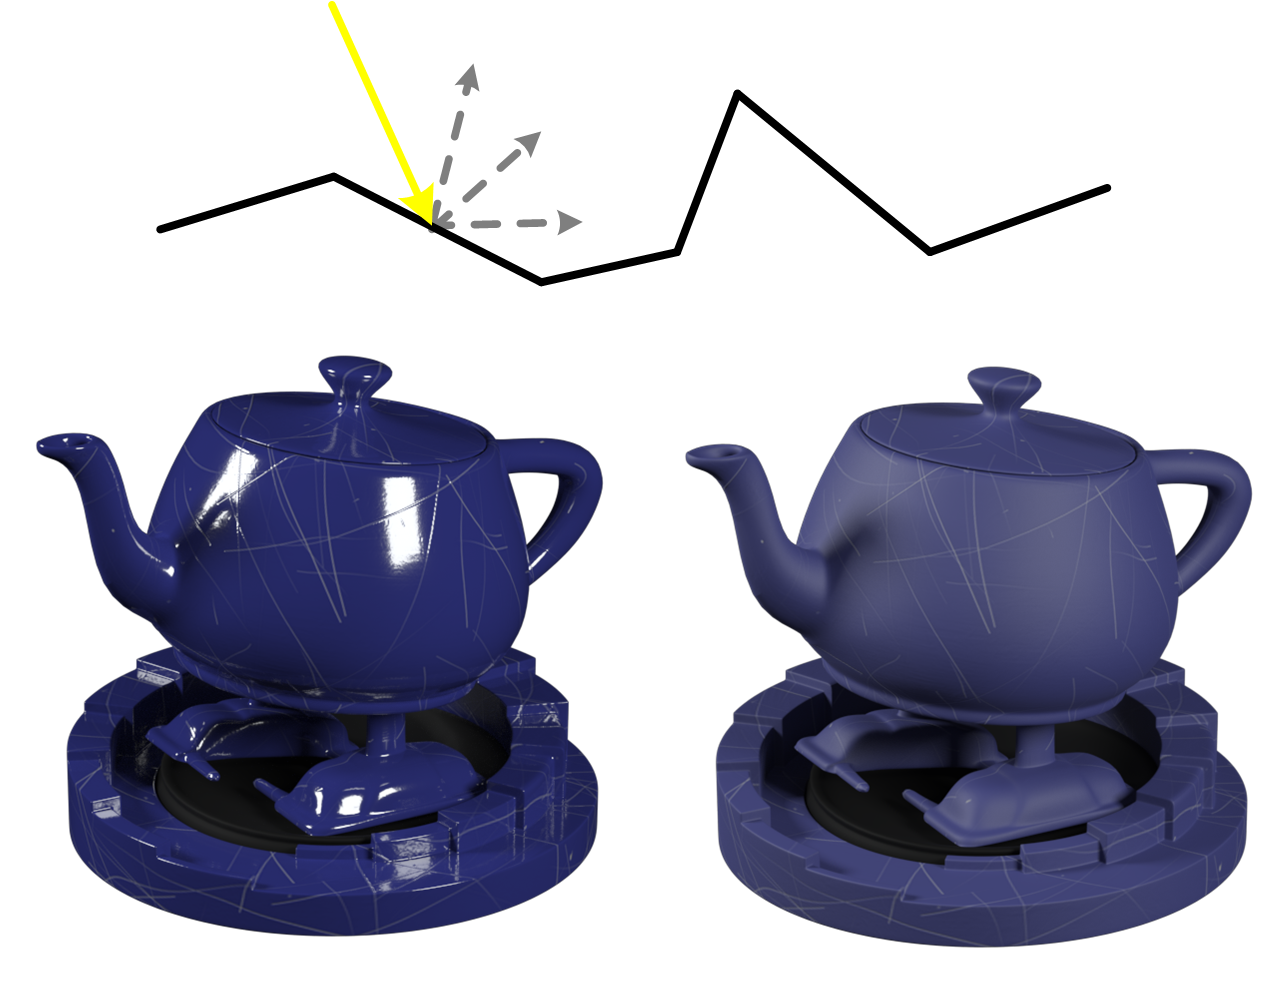
\includegraphics{figs/fundamentals/microfacets.png}
	\caption{Insight into microfacets of a surface. The striking energy reflects into the semisphere formed on the basis of the normal vector. Below, the same object rendered as a polished and rough surface. Therefore, the second present microfacets that lead to a wider energy scattering.}
	\label{fig:microfacets}
\end{marginfigure}
Analytical BRDFs have a large taxonomy if we attend to the kind of material and the criteria under which these were modelled. Although most of these aims to simulate a specific appearance (metal, wood, mats, polished surfaces, the Moon, etc.), materials are at least organized into isotropic and anisotropic materials. The first is invariant to rotations of the surface around $n$, whereas the second changes its reflection around $n$, emulating materials such as hair or brushed metal \cite{guarnera_brdf_2016}. On the other hand, BRDFs are categorized as phenomenological or empirical, physically-based or theoretical and data-driven. Phenomelogical include functions are computationally convenient methods for estimating the reflectance appearance of some materials, whereas theoretical make use of some attributes that intervene in physically-based shading. For instance, Phong was one of the first phenomenological models that were widely adopted with the advent of programmable pipelines. It is simply parameterized by the surface normal, $n$, lighting vector from a sole source, $l$, the view direction, $v$, and the reflection, $r$ computed according to the Fresnel law. On the other hand, Cook-Torrance is one, if not the most, representative theoretical BRDF as it pays attention to micro-facets, distinguished metal and dielectrics and uses the halfway vector, $h$, to compute the specular lobe. For novel CG programmers, this is frequently introduced as the foundational core of Physically-Based Rendering (PBR) for shader-based frameworks such as OpenGL. For further insight into analytical BRDFs, we refer the reader to explanations of these from a theoretical point of view \cite{guarnera_brdf_2016, soldado_overview_2012}. Note that radiance spreads over the hemisphere, and therefore, most of these functions include $\pi$ in the denominator and the numerator is scaled by the \verb|cosinus| function parameterized on $\omega_i$, $\omega_o$ and $n$. However, traditional CG applications avoid downscaling the computed intensity by $\pi$ since it darkens the rendered scene and they do not intend to behave as physically-based engines. 

\begin{figure}[!ht]
	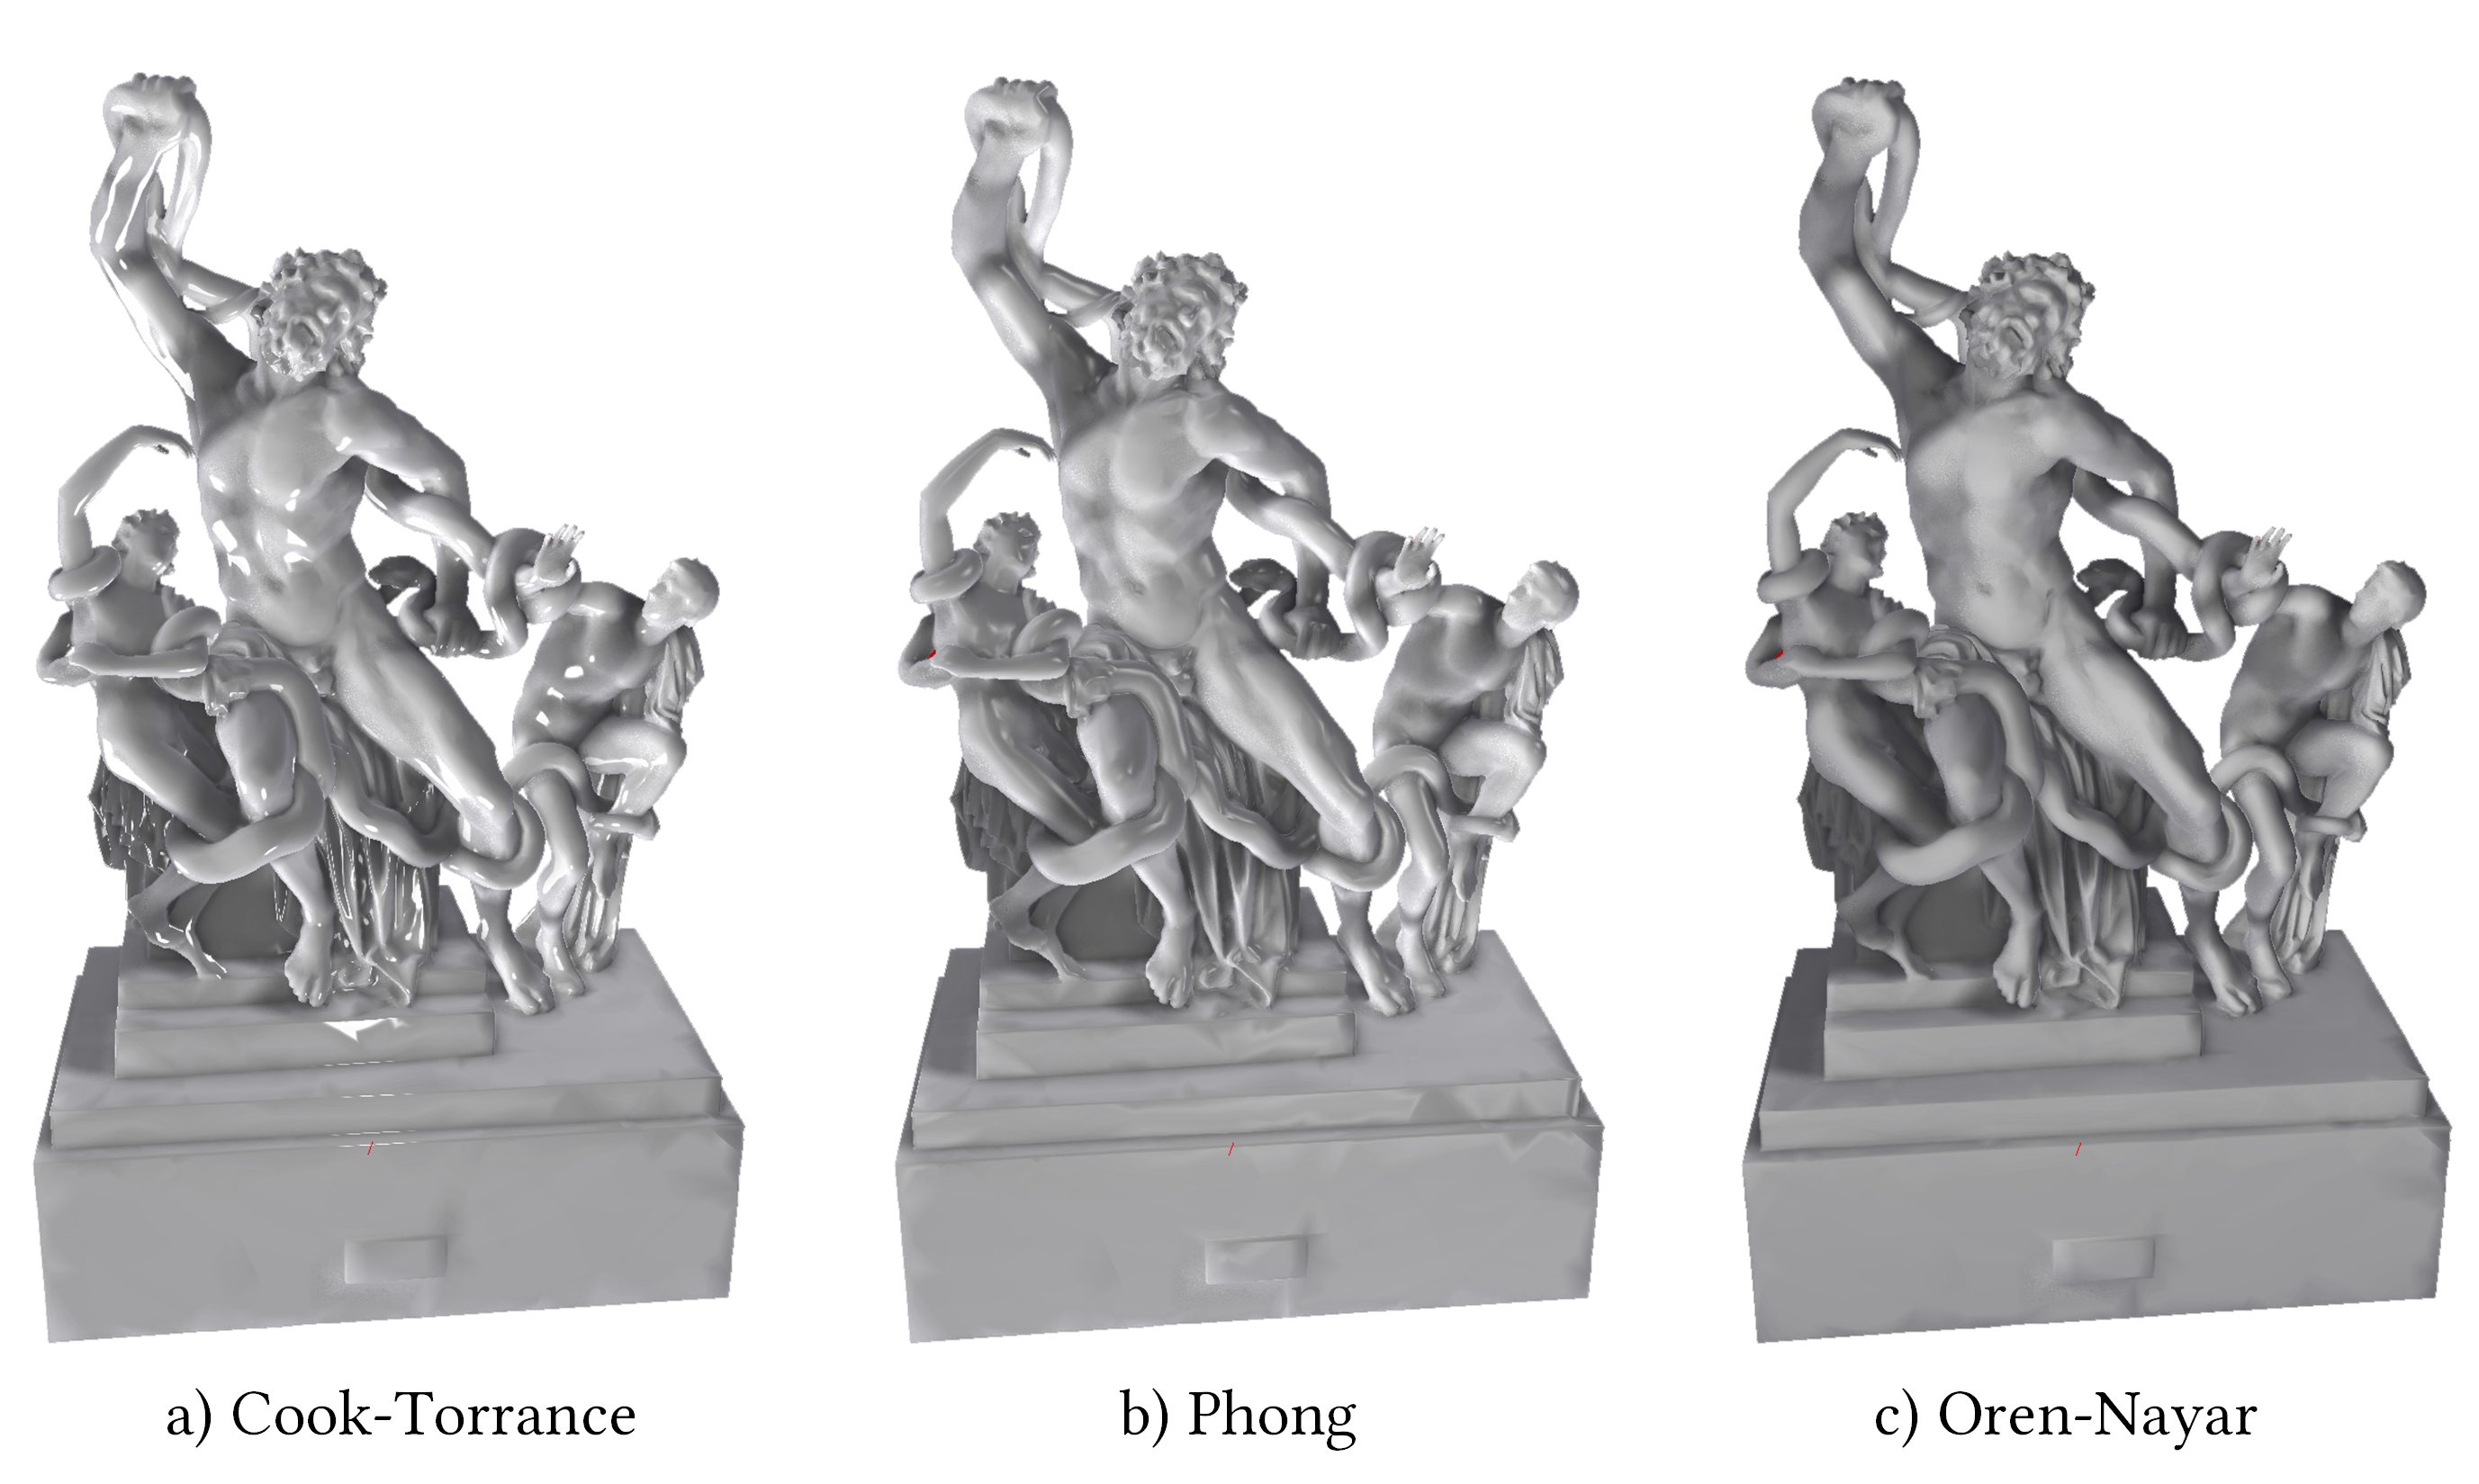
\includegraphics[width=\textwidth]{figs/fundamentals/analytical_brdf.png}
	\caption{Comparison of analytical BRDFS: a) Cook-Torrance ($f_0 \gets 1$, $\alpha \gets 0.077$), b) Phong ($ns \gets 32$) and c) Oren-Nayar ($\alpha \gets 0.75$). }
    \label{fig:analytical_brdf}
\end{figure}

\lstinputlisting[language=c++, caption={Minnaert BRDF implementation for a 1) reflectance visualization tool using a shemisphere and 2) a rendering application.}, label=code:analyticalbrdf]{code/minnaert.brdf}

% \begin{figure*}[!ht]
%     \imageannotated{figs/fundamentals/room_rt.png}{Hello world}{0}{-2.6}{white}
% 	\caption{Comparison of analytical BRDFS: a)  }
%     \label{fig:hello}
% \end{figure*}